
\chapter{Jueces}

\section*{Introducción al Libro de Jueces}

El \textbf{Libro de Jueces} es el segundo de los libros históricos del Antiguo Testamento y narra el período de transición entre la conquista de Canaán, liderada por Josué, y el establecimiento de la monarquía en Israel. Este libro recibe su nombre por los líderes carismáticos conocidos como \textbf{jueces}, quienes fueron levantados por Dios para guiar y liberar al pueblo de Israel en momentos de crisis.

\subsection*{Autoría}

La autoría del libro de Jueces es anónima, aunque tradicionalmente se ha atribuido al profeta Samuel. Sin embargo, estudios modernos sugieren que el texto fue compuesto y editado durante el período del exilio babilónico (siglo VI a.C.), probablemente por redactores deuteronomistas, quienes buscaron enfatizar la obediencia a Dios como clave para la estabilidad de Israel.

\subsection*{Temática}

El libro de Jueces está estructurado en ciclos narrativos que describen el constante patrón de infidelidad y redención del pueblo de Israel. Sus temas principales incluyen:
\begin{itemize}
	\item \textbf{La infidelidad de Israel:} El pueblo abandona a Dios para adorar a dioses extranjeros, rompiendo el pacto establecido.
	\item \textbf{La opresión extranjera:} Como consecuencia de su pecado, Israel es sometido por pueblos vecinos.
	\item \textbf{El clamor por liberación:} En su angustia, el pueblo clama a Dios, quien responde levantando jueces para liberarlos.
	\item \textbf{El liderazgo de los jueces:} Figuras como Débora, Gedeón, Jefté y Sansón desempeñan un papel central como líderes militares y espirituales, aunque con defectos humanos.
	\item \textbf{El ciclo de desobediencia:} Tras la muerte de cada juez, el pueblo vuelve a caer en idolatría, reiniciando el ciclo de opresión y redención.
\end{itemize}



El contexto histórico del libro de Jueces refleja un período de descentralización política y religiosa en Israel. Sin un líder unificador como Moisés o Josué, las tribus actuaban de manera independiente, enfrentando constantes amenazas de los pueblos circundantes, como los filisteos, los madianitas y los cananeos. Este tiempo de inestabilidad destaca la necesidad de una guía divina para el pueblo de Israel.



El libro de Jueces ilustra la fragilidad humana y la fidelidad de Dios. A través de los relatos de los jueces, el libro subraya el poder de Dios para salvar y restaurar incluso en medio de la debilidad y el pecado del pueblo. Además, sirve como un preludio a la instauración de la monarquía en Israel, destacando la necesidad de un liderazgo firme y fiel a Dios.\\





\begin{center}
	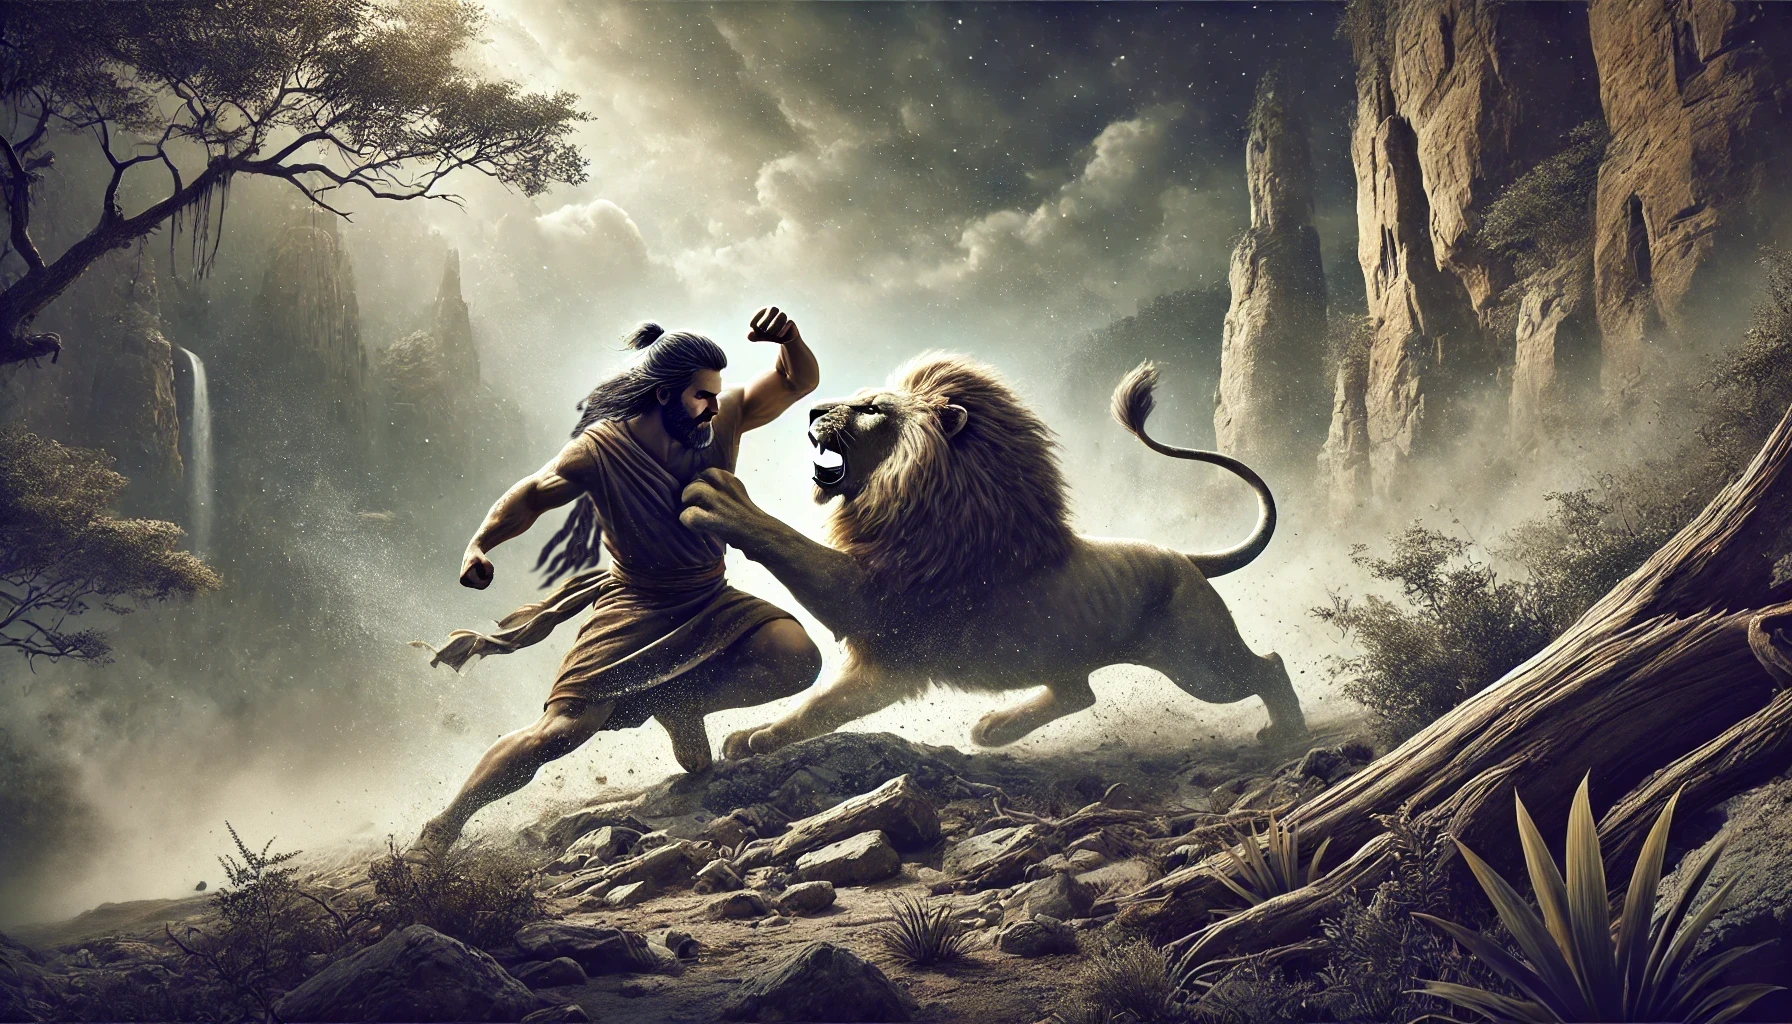
\includegraphics[width=0.7\linewidth]{graficas/jueses}\\
	Sansón contra el León\\
\end{center}


\section*{Capítulo 1}
Judá y Simeón capturan a Adoni-bezec  

1:1 Aconteció después de la muerte de Josué, que los hijos de Israel consultaron a Jehová, diciendo: ¿Quién de nosotros subirá primero a pelear contra los cananeos?  
1:2 Y Jehová respondió: Judá subirá; he aquí que yo he entregado la tierra en sus manos.  
1:3 Y Judá dijo a Simeón su hermano: Sube conmigo al territorio que se me ha adjudicado, y peleemos contra el cananeo, y yo también iré contigo al tuyo. Y Simeón fue con él.  
1:4 Y subió Judá, y Jehová entregó en sus manos al cananeo y al ferezeo; e hirieron de ellos en Bezec a diez mil hombres.  
1:5 Y hallaron a Adoni-bezec en Bezec, y pelearon contra él; y derrotaron al cananeo y al ferezeo.  
1:6 Mas Adoni-bezec huyó; y le siguieron y le prendieron, y le cortaron los pulgares de las manos y de los pies.  
1:7 Entonces dijo Adoni-bezec: Setenta reyes, cortados los pulgares de sus manos y de sus pies, recogían las migajas debajo de mi mesa; como yo hice, así me ha pagado Dios. Y le llevaron a Jerusalén, donde murió.  
Judá conquista Jerusalén y Hebrón  
1:8 Y combatieron los hijos de Judá a Jerusalén y la tomaron, y pasaron a sus habitantes a filo de espada y pusieron fuego a la ciudad.  
1:9 Después los hijos de Judá descendieron para pelear contra el cananeo que habitaba en las montañas, en el Neguev, y en los llanos.  
1:10 Y marchó Judá contra el cananeo que habitaba en Hebrón, la cual se llamaba antes Quiriat-arba; e hirieron a Sesai, a Ahimán y a Talmai.  
Otoniel conquista Debir y recibe a Acsa   
1:11 De allí fue a los que habitaban en Debir, que antes se llamaba Quiriat-sefer. 
1:12 Y dijo Caleb: El que atacare a Quiriat-sefer y la tomare, yo le daré Acsa mi hija por mujer.  
1:13 Y la tomó Otoniel hijo de Cenaz, hermano menor de Caleb; y él le dio Acsa su hija por mujer.  
1:14 Y cuando ella se iba con él, la persuadió que pidiese a su padre un campo. Y ella se bajó del asno, y Caleb le dijo: ¿Qué tienes?  
1:15 Ella entonces le respondió: Concédeme un don; puesto que me has dado tierra del Neguev, dame también fuentes de aguas. Entonces Caleb le dio las fuentes de arriba y las fuentes de abajo.  
Extensión de las conquistas de Judá y de Benjamín  
1:16 Y los hijos del ceneo, suegro de Moisés, subieron de la ciudad de las palmeras con los hijos de Judá al desierto de Judá, que está en el Neguev cerca de Arad; y fueron y habitaron con el pueblo.  
1:17 Y fue Judá con su hermano Simeón, y derrotaron al cananeo que habitaba en Sefat, y la asolaron; y pusieron por nombre a la ciudad, Horma.  
1:18 Tomó también Judá a Gaza con su territorio, Ascalón con su territorio y Ecrón con su territorio.  
1:19 Y Jehová estaba con Judá, quien arrojó a los de las montañas; mas no pudo arrojar a los que habitaban en los llanos, los cuales tenían carros herrados.  
1:20 Y dieron Hebrón a Caleb, como Moisés había dicho; y él arrojó de allí a los tres hijos de Anac. 
1:21 Mas al jebuseo que habitaba en Jerusalén no lo arrojaron los hijos de Benjamín, y el jebuseo habitó con los hijos de Benjamín en Jerusalén hasta hoy. 
José conquista Bet-el  
1:22 También la casa de José subió contra Bet-el; y Jehová estaba con ellos.  
1:23 Y la casa de José puso espías en Bet-el, ciudad que antes se llamaba Luz.  
1:24 Y los que espiaban vieron a un hombre que salía de la ciudad, y le dijeron: Muéstranos ahora la entrada de la ciudad, y haremos contigo misericordia.  
1:25 Y él les mostró la entrada a la ciudad, y la hirieron a filo de espada; pero dejaron ir a aquel hombre con toda su familia.  
1:26 Y se fue el hombre a la tierra de los heteos, y edificó una ciudad a la cual llamó Luz; y este es su nombre hasta hoy.  
Extensión de las conquistas de Manasés y de Efraín  
1:27 Tampoco Manasés arrojó a los de Bet-seán, ni a los de sus aldeas, ni a los de Taanac y sus aldeas, ni a los de Dor y sus aldeas, ni a los habitantes de Ibleam y sus aldeas, ni a los que habitan en Meguido y en sus aldeas; y el cananeo persistía en habitar en aquella tierra.  
1:28 Pero cuando Israel se sintió fuerte hizo al cananeo tributario, mas no lo arrojó. 
1:29 Tampoco Efraín arrojó al cananeo que habitaba en Gezer, sino que habitó el cananeo en medio de ellos en Gezer. 
Extensión de las conquistas de las demás tribus  
1:30 Tampoco Zabulón arrojó a los que habitaban en Quitrón, ni a los que habitaban en Naalal, sino que el cananeo habitó en medio de él, y le fue tributario.  
1:31 Tampoco Aser arrojó a los que habitaban en Aco, ni a los que habitaban en Sidón, en Ahlab, en Aczib, en Helba, en Afec y en Rehob.  
1:32 Y moró Aser entre los cananeos que habitaban en la tierra; pues no los arrojó.  
1:33 Tampoco Neftalí arrojó a los que habitaban en Bet-semes, ni a los que habitaban en Bet-anat, sino que moró entre los cananeos que habitaban en la tierra; mas le fueron tributarios los moradores de Bet-semes y los moradores de Bet-anat. 
1:34 Los amorreos acosaron a los hijos de Dan hasta el monte, y no los dejaron descender a los llanos.  
1:35 Y el amorreo persistió en habitar en el monte de Heres, en Ajalón y en Saalbim; pero cuando la casa de José cobró fuerzas, lo hizo tributario.  
1:36 Y el límite del amorreo fue desde la subida de Acrabim, desde Sela hacia arriba.  
\section*{Capítulo 2}
El ángel de Jehová en Boquim  

2:1 El ángel de Jehová subió de Gilgal a Boquim, y dijo: Yo os saqué de Egipto, y os introduje en la tierra de la cual había jurado a vuestros padres, diciendo: No invalidaré jamás mi pacto con vosotros,  
2:2 con tal que vosotros no hagáis pacto con los moradores de esta tierra, cuyos altares habéis de derribar; mas vosotros no habéis atendido a mi voz. ¿Por qué habéis hecho esto?  
2:3 Por tanto, yo también digo: No los echaré de delante de vosotros, sino que serán azotes para vuestros costados, y sus dioses os serán tropezadero.  
2:4 Cuando el ángel de Jehová habló estas palabras a todos los hijos de Israel, el pueblo alzó su voz y lloró.  
2:5 Y llamaron el nombre de aquel lugar Boquim, y ofrecieron allí sacrificios a Jehová.  
Muerte de Josué   
2:6 Porque ya Josué había despedido al pueblo, y los hijos de Israel se habían ido cada uno a su heredad para poseerla.  
2:7 Y el pueblo había servido a Jehová todo el tiempo de Josué, y todo el tiempo de los ancianos que sobrevivieron a Josué, los cuales habían visto todas las grandes obras de Jehová, que él había hecho por Israel.  
2:8 Pero murió Josué hijo de Nun, siervo de Jehová, siendo de ciento diez años.  
2:9 Y lo sepultaron en su heredad en Timnat-sera, en el monte de Efraín, al norte del monte de Gaas.  
2:10 Y toda aquella generación también fue reunida a sus padres. Y se levantó después de ellos otra generación que no conocía a Jehová, ni la obra que él había hecho por Israel.  
Apostasía de Israel, y la obra de los jueces  
2:11 Después los hijos de Israel hicieron lo malo ante los ojos de Jehová, y sirvieron a los baales.  
2:12 Dejaron a Jehová el Dios de sus padres, que los había sacado de la tierra de Egipto, y se fueron tras otros dioses, los dioses de los pueblos que estaban en sus alrededores, a los cuales adoraron; y provocaron a ira a Jehová.  
2:13 Y dejaron a Jehová, y adoraron a Baal y a Astarot.  
2:14 Y se encendió contra Israel el furor de Jehová, el cual los entregó en manos de robadores que los despojaron, y los vendió en mano de sus enemigos de alrededor; y no pudieron ya hacer frente a sus enemigos.  
2:15 Por dondequiera que salían, la mano de Jehová estaba contra ellos para mal, como Jehová había dicho, y como Jehová se lo había jurado; y tuvieron gran aflicción.  
2:16 Y Jehová levantó jueces que los librasen de mano de los que les despojaban;  
2:17 pero tampoco oyeron a sus jueces, sino que fueron tras dioses ajenos, a los cuales adoraron; se apartaron pronto del camino en que anduvieron sus padres obedeciendo a los mandamientos de Jehová; ellos no hicieron así.  
2:18 Y cuando Jehová les levantaba jueces, Jehová estaba con el juez, y los libraba de mano de los enemigos todo el tiempo de aquel juez; porque Jehová era movido a misericordia por sus gemidos a causa de los que los oprimían y afligían. 
2:19 Mas acontecía que al morir el juez, ellos volvían atrás, y se corrompían más que sus padres, siguiendo a dioses ajenos para servirles, e inclinándose delante de ellos; y no se apartaban de sus obras, ni de su obstinado camino.  
2:20 Y la ira de Jehová se encendió contra Israel, y dijo: Por cuanto este pueblo traspasa mi pacto que ordené a sus padres, y no obedece a mi voz,  
2:21 tampoco yo volveré más a arrojar de delante de ellos a ninguna de las naciones que dejó Josué cuando murió;  
2:22 para probar con ellas a Israel, si procurarían o no seguir el camino de Jehová, andando en él, como lo siguieron sus padres.  
2:23 Por esto dejó Jehová a aquellas naciones, sin arrojarlas de una vez, y no las entregó en mano de Josué.  
\section*{Capítulo 3}
Naciones que fueron dejadas para probar a Israel  

3:1 Estas, pues, son las naciones que dejó Jehová para probar con ellas a Israel, a todos aquellos que no habían conocido todas la guerras de Canaán;  
3:2 solamente para que el linaje de los hijos de Israel conociese la guerra, para que la enseñasen a los que antes no la habían conocido:  
3:3 los cinco príncipes de los filisteos, todos los cananeos, los sidonios, y los heveos que habitaban en el monte Líbano, desde el monte de Baal-hermón hasta llegar a Hamat.  
3:4 Y fueron para probar con ellos a Israel, para saber si obedecerían a los mandamientos de Jehová, que él había dado a sus padres por mano de Moisés.  
3:5 Así los hijos de Israel habitaban entre los cananeos, heteos, amorreos, ferezeos, heveos y jebuseos.  
3:6 Y tomaron de sus hijas por mujeres, y dieron sus hijas a los hijos de ellos, y sirvieron a sus dioses.  
Otoniel liberta a Israel de Cusan-risataim  
3:7 Hicieron, pues, los hijos de Israel lo malo ante los ojos de Jehová, y olvidaron a Jehová su Dios, y sirvieron a los baales y a las imágenes de Asera.  
3:8 Y la ira de Jehová se encendió contra Israel, y los vendió en manos de Cusan-risataim rey de Mesopotamia; y sirvieron los hijos de Israel a Cusan-risataim ocho años.  
3:9 Entonces clamaron los hijos de Israel a Jehová; y Jehová levantó un libertador a los hijos de Israel y los libró; esto es, a Otoniel hijo de Cenaz, hermano menor de Caleb.  
3:10 Y el Espíritu de Jehová vino sobre él, y juzgó a Israel, y salió a batalla, y Jehová entregó en su mano a Cusan-risataim rey de Siria, y prevaleció su mano contra Cusan-risataim.  
3:11 Y reposó la tierra cuarenta años; y murió Otoniel hijo de Cenaz.  
Aod liberta a Israel de Moab  
3:12 Volvieron los hijos de Israel a hacer lo malo ante los ojos de Jehová; y Jehová fortaleció a Eglón rey de Moab contra Israel, por cuanto habían hecho lo malo ante los ojos de Jehová.  
3:13 Este juntó consigo a los hijos de Amón y de Amalec, y vino e hirió a Israel, y tomó la ciudad de las palmeras.  
3:14 Y sirvieron los hijos de Israel a Eglón rey de los moabitas dieciocho años.  
3:15 Y clamaron los hijos de Israel a Jehová; y Jehová les levantó un libertador, a Aod hijo de Gera, benjamita, el cual era zurdo. Y los hijos de Israel enviaron con él un presente a Eglón rey de Moab.  
3:16 Y Aod se había hecho un puñal de dos filos, de un codo  de largo; y se lo ciñó debajo de sus vestidos a su lado derecho.  
3:17 Y entregó el presente a Eglón rey de Moab; y era Eglón hombre muy grueso.  
3:18 Y luego que hubo entregado el presente, despidió a la gente que lo había traído.  
3:19 Mas él se volvió desde los ídolos que están en Gilgal, y dijo: Rey, una palabra secreta tengo que decirte. El entonces dijo: Calla. Y salieron de delante de él todos los que con él estaban.  
3:20 Y se le acercó Aod, estando él sentado solo en su sala de verano. Y Aod dijo: Tengo palabra de Dios para ti. El entonces se levantó de la silla.  
3:21 Entonces alargó Aod su mano izquierda, y tomó el puñal de su lado derecho, y se lo metió por el vientre,  
3:22 de tal manera que la empuñadura entró también tras la hoja, y la gordura cubrió la hoja, porque no sacó el puñal de su vientre; y salió el estiércol.  
3:23 Y salió Aod al corredor, y cerró tras sí las puertas de la sala y las aseguró con el cerrojo.  
3:24 Cuando él hubo salido, vinieron los siervos del rey, los cuales viendo las puertas de la sala cerradas, dijeron: Sin duda él cubre sus pies en la sala de verano.  
3:25 Y habiendo esperado hasta estar confusos, porque él no abría las puertas de la sala, tomaron la llave y abrieron; y he aquí su señor caído en tierra, muerto.  
3:26 Mas entre tanto que ellos se detuvieron, Aod escapó, y pasando los ídolos, se puso a salvo en Seirat.  
3:27 Y cuando había entrado, tocó el cuerno en el monte de Efraín, y los hijos de Israel descendieron con él del monte, y él iba delante de ellos.  
3:28 Entonces él les dijo: Seguidme, porque Jehová ha entregado a vuestros enemigos los moabitas en vuestras manos. Y descendieron en pos de él, y tomaron los vados del Jordán a Moab, y no dejaron pasar a ninguno.  
3:29 Y en aquel tiempo mataron de los moabitas como diez mil hombres, todos valientes y todos hombres de guerra; no escapó ninguno.  
3:30 Así fue subyugado Moab aquel día bajo la mano de Israel; y reposó la tierra ochenta años.  
Samgar liberta a Israel de los filisteos  
3:31 Después de él fue Samgar hijo de Anat, el cual mató a seiscientos hombres de los filisteos con una aguijada de bueyes; y él también salvó a Israel.  
\section*{Capítulo 4 }
Débora y Barac derrotan a Sísara  

4:1 Después de la muerte de Aod, los hijos de Israel volvieron a hacer lo malo ante los ojos de Jehová.  
4:2 Y Jehová los vendió en mano de Jabín rey de Canaán, el cual reinó en Hazor; y el capitán de su ejército se llamaba Sísara, el cual habitaba en Haroset-goim.  
4:3 Entonces los hijos de Israel clamaron a Jehová, porque aquél tenía novecientos carros herrados, y había oprimido con crueldad a los hijos de Israel por veinte años.  
4:4 Gobernaba en aquel tiempo a Israel una mujer, Débora, profetisa, mujer de Lapidot;  
4:5 y acostumbraba sentarse bajo la palmera de Débora, entre Ramá y Bet-el, en el monte de Efraín; y los hijos de Israel subían a ella a juicio.  
4:6 Y ella envió a llamar a Barac hijo de Abinoam, de Cedes de Neftalí, y le dijo: ¿No te ha mandado Jehová Dios de Israel, diciendo: Ve, junta a tu gente en el monte de Tabor, y toma contigo diez mil hombres de la tribu de Neftalí y de la tribu de Zabulón;  
4:7 y yo atraeré hacia ti al arroyo de Cisón a Sísara, capitán del ejército de Jabín, con sus carros y su ejército, y lo entregaré en tus manos?  
4:8 Barac le respondió: Si tú fueres conmigo, yo iré; pero si no fueres conmigo, no iré.  
4:9 Ella dijo: Iré contigo; mas no será tuya la gloria de la jornada que emprendes, porque en mano de mujer venderá Jehová a Sísara. Y levantándose Débora, fue con Barac a Cedes.  
4:10 Y juntó Barac a Zabulón y a Neftalí en Cedes, y subió con diez mil hombres a su mando; y Débora subió con él.  
4:11 Y Heber ceneo, de los hijos de Hobab suegro de Moisés, se había apartado de los ceneos, y había plantado sus tiendas en el valle de Zaanaim, que está junto a Cedes.  
4:12 Vinieron, pues, a Sísara las nuevas de que Barac hijo de Abinoam había subido al monte de Tabor.  
4:13 Y reunió Sísara todos sus carros, novecientos carros herrados, con todo el pueblo que con él estaba, desde Haroset- goim hasta el arroyo de Cisón.  
4:14 Entonces Débora dijo a Barac: Levántate, porque este es el día en que Jehová ha entregado a Sísara en tus manos. ¿No ha salido Jehová delante de ti? Y Barac descendió del monte de Tabor, y diez mil hombres en pos de él.  
4:15 Y Jehová quebrantó a Sísara, a todos sus carros y a todo su ejército, a filo de espada delante de Barac; y Sísara descendió del carro, y huyó a pie.  
4:16 Mas Barac siguió los carros y el ejército hasta Haroset- goim, y todo el ejército de Sísara cayó a filo de espada, hasta no quedar ni uno.  
4:17 Y Sísara huyó a pie a la tienda de Jael mujer de Heber ceneo; porque había paz entre Jabín rey de Hazor y la casa de Heber ceneo.  
4:18 Y saliendo Jael a recibir a Sísara, le dijo: Ven, señor mío, ven a mí, no tengas temor. Y él vino a ella a la tienda, y ella le cubrió con una manta.  
4:19 Y él le dijo: Te ruego me des de beber un poco de agua, pues tengo sed. Y ella abrió un odre de leche y le dio de beber, y le volvió a cubrir.  
4:20 Y él le dijo: Estate a la puerta de la tienda; y si alguien viniere, y te preguntare, diciendo: ¿Hay aquí alguno? tú responderás que no.  
4:21 Pero Jael mujer de Heber tomó una estaca de la tienda, y poniendo un mazo en su mano, se le acercó calladamente y le metió la estaca por las sienes, y la enclavó en la tierra, pues él estaba cargado de sueño y cansado; y así murió.  
4:22 Y siguiendo Barac a Sísara, Jael salió a recibirlo, y le dijo: Ven, y te mostraré al varón que tú buscas. Y él entró donde ella estaba, y he aquí Sísara yacía muerto con la estaca por la sien.  
4:23 Así abatió Dios aquel día a Jabín, rey de Canaán, delante de los hijos de Israel.  
4:24 Y la mano de los hijos de Israel fue endureciéndose más y más contra Jabín rey de Canaán, hasta que lo destruyeron.  
\section*{Capítulo 5}
Cántico de Débora y de Barac  

5:1 Aquel día cantó Débora con Barac hijo de Abinoam, diciendo:  
5:2 Por haberse puesto al frente los caudillos en Israel,  
Por haberse ofrecido voluntariamente el pueblo,  
Load a Jehová.  
5:3 Oíd, reyes; escuchad, oh príncipes;  
Yo cantaré a Jehová,  
Cantaré salmos a Jehová, el Dios de Israel.  
5:4 Cuando saliste de Seir, oh Jehová,  
Cuando te marchaste de los campos de Edom,  
La tierra tembló, y los cielos destilaron,  
Y las nubes gotearon aguas. 
5:5 Los montes temblaron delante de Jehová,  
Aquel Sinaí, delante de Jehová Dios de Israel. 
5:6 En los días de Samgar hijo de Anat,  
En los días de Jael, quedaron abandonados los caminos,  
Y los que andaban por las sendas se apartaban por senderos torcidos.  
5:7 Las aldeas quedaron abandonadas en Israel, habían decaído,  
Hasta que yo Débora me levanté,  
Me levanté como madre en Israel. 
5:8 Cuando escogían nuevos dioses,  
La guerra estaba a las puertas;  
¿Se veía escudo o lanza  
Entre cuarenta mil en Israel? 
5:9 Mi corazón es para vosotros, jefes de Israel,  
Para los que voluntariamente os ofrecisteis entre el pueblo.  
Load a Jehová.  
5:10 Vosotros los que cabalgáis en asnas blancas,  
Los que presidís en juicio,  
Y vosotros los que viajáis, hablad.  
5:11 Lejos del ruido de los arqueros, en los abrevaderos,  
Allí repetirán los triunfos de Jehová,  
Los triunfos de sus aldeas en Israel;  
Entonces marchará hacia las puertas el pueblo de Jehová.  
5:12 Despierta, despierta, Débora;  
Despierta, despierta, entona cántico.  
Levántate, Barac, y lleva tus cautivos, hijo de Abinoam.  
5:13 Entonces marchó el resto de los nobles;  
El pueblo de Jehová marchó por él en contra de los poderosos.  
5:14 De Efraín vinieron los radicados en Amalec,  
En pos de ti, Benjamín, entre tus pueblos;  
De Maquir descendieron príncipes,  
Y de Zabulón los que tenían vara de mando.  
5:15 Caudillos también de Isacar fueron con Débora;  
Y como Barac, también Isacar  
Se precipitó a pie en el valle.  
Entre las familias de Rubén  
Hubo grandes resoluciones del corazón.  
5:16 ¿Por qué te quedaste entre los rediles,  
Para oír los balidos de los rebaños?  
Entre las familias de Rubén  
Hubo grandes propósitos del corazón. 
5:17 Galaad se quedó al otro lado del Jordán;  
Y Dan, ¿por qué se estuvo junto a las naves?  
Se mantuvo Aser a la ribera del mar,  
Y se quedó en sus puertos.  
5:18 El pueblo de Zabulón expuso su vida a la muerte,  
Y Neftalí en las alturas del campo.  
5:19 Vinieron reyes y pelearon;  
Entonces pelearon los reyes de Canaán,  
En Taanac, junto a las aguas de Meguido,  
Mas no llevaron ganancia alguna de dinero.  
5:20 Desde los cielos pelearon las estrellas;  
Desde sus órbitas pelearon contra Sísara.  
5:21 Los barrió el torrente de Cisón,  
El antiguo torrente, el torrente de Cisón.  
Marcha, oh alma mía, con poder.  
5:22 Entonces resonaron los cascos de los caballos  
Por el galopar, por el galopar de sus valientes.  
5:23 Maldecid a Meroz, dijo el ángel de Jehová;  
Maldecid severamente a sus moradores,  
Porque no vinieron al socorro de Jehová,  
Al socorro de Jehová contra los fuertes.  
5:24 Bendita sea entre las mujeres Jael,  
Mujer de Heber ceneo;  
Sobre las mujeres bendita sea en la tienda.  
5:25 El pidió agua, y ella le dio leche; 
En tazón de nobles le presentó crema.  
5:26 Tendió su mano a la estaca,  
Y su diestra al mazo de trabajadores,  
Y golpeó a Sísara; hirió su cabeza,  
Y le horadó, y atravesó sus sienes. 
5:27 Cayó encorvado entre sus pies, quedó tendido;  
Entre sus pies cayó encorvado;  
Donde se encorvó, allí cayó muerto.  
5:28 La madre de Sísara se asoma a la ventana,  
Y por entre las celosías a voces dice:  
¿Por qué tarda su carro en venir?  
¿Por qué las ruedas de sus carros se detienen?  
5:29 Las más avisadas de sus damas le respondían,  
Y aun ella se respondía a sí misma:  
5:30 ¿No han hallado botín, y lo están repartiendo?  
A cada uno una doncella, o dos;  
Las vestiduras de colores para Sísara,  
Las vestiduras bordadas de colores;  
La ropa de color bordada de ambos lados, para los jefes de los que tomaron el botín.  
5:31 Así perezcan todos tus enemigos, oh Jehová;  
Mas los que te aman, sean como el sol cuando sale en su fuerza.  
Y la tierra reposó cuarenta años.  
\section*{Capítulo 6}
Llamamiento de Gedeón  

6:1 Los hijos de Israel hicieron lo malo ante los ojos de Jehová; y Jehová los entregó en mano de Madián por siete años.  
6:2 Y la mano de Madián prevaleció contra Israel. Y los hijos de Israel, por causa de los madianitas, se hicieron cuevas en los montes, y cavernas, y lugares fortificados.  
6:3 Pues sucedía que cuando Israel había sembrado, subían los madianitas y amalecitas y los hijos del oriente contra ellos; subían y los atacaban.  
6:4 Y acampando contra ellos destruían los frutos de la tierra, hasta llegar a Gaza; y no dejaban qué comer en Israel, ni ovejas, ni bueyes, ni asnos.  
6:5 Porque subían ellos y sus ganados, y venían con sus tiendas en grande multitud como langostas; ellos y sus camellos eran innumerables; así venían a la tierra para devastarla.  
6:6 De este modo empobrecía Israel en gran manera por causa de Madián; y los hijos de Israel clamaron a Jehová.  
6:7 Y cuando los hijos de Israel clamaron a Jehová, a causa de los madianitas,  
6:8 Jehová envió a los hijos de Israel un varón profeta, el cual les dijo: Así ha dicho Jehová Dios de Israel: Yo os hice salir de Egipto, y os saqué de la casa de servidumbre.  
6:9 Os libré de mano de los egipcios, y de mano de todos los que os afligieron, a los cuales eché de delante de vosotros, y os di su tierra;  
6:10 y os dije: Yo soy Jehová vuestro Dios; no temáis a los dioses de los amorreos, en cuya tierra habitáis; pero no habéis obedecido a mi voz.  
6:11 Y vino el ángel de Jehová, y se sentó debajo de la encina que está en Ofra, la cual era de Joás abiezerita; y su hijo Gedeón estaba sacudiendo el trigo en el lagar, para esconderlo de los madianitas.  
6:12 Y el ángel de Jehová se le apareció, y le dijo: Jehová está contigo, varón esforzado y valiente.  
6:13 Y Gedeón le respondió: Ah, señor mío, si Jehová está con nosotros, ¿por qué nos ha sobrevenido todo esto? ¿Y dónde están todas sus maravillas, que nuestros padres nos han contado, diciendo: ¿No nos sacó Jehová de Egipto? Y ahora Jehová nos ha desamparado, y nos ha entregado en mano de los madianitas.  
6:14 Y mirándole Jehová, le dijo: Ve con esta tu fuerza, y salvarás a Israel de la mano de los madianitas. ¿No te envío yo?  
6:15 Entonces le respondió: Ah, señor mío, ¿con qué salvaré yo a Israel? He aquí que mi familia es pobre en Manasés, y yo el menor en la casa de mi padre.  
6:16 Jehová le dijo: Ciertamente yo estaré contigo, y derrotarás a los madianitas como a un solo hombre.  
6:17 Y él respondió: Yo te ruego que si he hallado gracia delante de ti, me des señal de que tú has hablado conmigo.  
6:18 Te ruego que no te vayas de aquí hasta que vuelva a ti, y saque mi ofrenda y la ponga delante de ti. Y él respondió: Yo esperaré hasta que vuelvas.  
6:19 Y entrando Gedeón, preparó un cabrito, y panes sin levadura de un efa  de harina; y puso la carne en un canastillo, y el caldo en una olla, y sacándolo se lo presentó debajo de aquella encina.  
6:20 Entonces el ángel de Dios le dijo: Toma la carne y los panes sin levadura, y ponlos sobre esta peña, y vierte el caldo. Y él lo hizo así.  
6:21 Y extendiendo el ángel de Jehová el báculo que tenía en su mano, tocó con la punta la carne y los panes sin levadura; y subió fuego de la peña, el cual consumió la carne y los panes sin levadura. Y el ángel de Jehová desapareció de su vista.  
6:22 Viendo entonces Gedeón que era el ángel de Jehová, dijo: Ah, Señor Jehová, que he visto al ángel de Jehová cara a cara. 
6:23 Pero Jehová le dijo: Paz a ti; no tengas temor, no morirás.  
6:24 Y edificó allí Gedeón altar a Jehová, y lo llamó Jehová-salom; el cual permanece hasta hoy en Ofra de los abiezeritas.  
6:25 Aconteció que la misma noche le dijo Jehová: Toma un toro del hato de tu padre, el segundo toro de siete años, y derriba el altar de Baal que tu padre tiene, y corta también la imagen de Asera que está junto a él;  
6:26 y edifica altar a Jehová tu Dios en la cumbre de este peñasco en lugar conveniente; y tomando el segundo toro, sacrifícalo en holocausto con la madera de la imagen de Asera que habrás cortado.  
6:27 Entonces Gedeón tomó diez hombres de sus siervos, e hizo como Jehová le dijo. Mas temiendo hacerlo de día, por la familia de su padre y por los hombres de la ciudad, lo hizo de noche.  
6:28 Por la mañana, cuando los de la ciudad se levantaron, he aquí que el altar de Baal estaba derribado, y cortada la imagen de Asera que estaba junto a él, y el segundo toro había sido ofrecido en holocausto sobre el altar edificado.  
6:29 Y se dijeron unos a otros: ¿Quién ha hecho esto? Y buscando e inquiriendo, les dijeron: Gedeón hijo de Joás lo ha hecho. Entonces los hombres de la ciudad dijeron a Joás:  
6:30 Saca a tu hijo para que muera, porque ha derribado el altar de Baal y ha cortado la imagen de Asera que estaba junto a él.  
6:31 Y Joás respondió a todos los que estaban junto a él: ¿Contenderéis vosotros por Baal? ¿Defenderéis su causa? Cualquiera que contienda por él, que muera esta mañana. Si es un dios, contienda por sí mismo con el que derribó su altar.  
6:32 Aquel día Gedeón fue llamado Jerobaal, esto es: Contienda Baal contra él, por cuanto derribó su altar.  
6:33 Pero todos los madianitas y amalecitas y los del oriente se juntaron a una, y pasando acamparon en el valle de Jezreel.  
6:34 Entonces el Espíritu de Jehová vino sobre Gedeón, y cuando éste tocó el cuerno, los abiezeritas se reunieron con él.  
6:35 Y envió mensajeros por todo Manasés, y ellos también se juntaron con él; asimismo envió mensajeros a Aser, a Zabulón y a Neftalí, los cuales salieron a encontrarles.  
6:36 Y Gedeón dijo a Dios: Si has de salvar a Israel por mi mano, como has dicho,  
6:37 he aquí que yo pondré un vellón de lana en la era; y si el rocío estuviere en el vellón solamente, quedando seca toda la otra tierra, entonces entenderé que salvarás a Israel por mi mano, como lo has dicho.  
6:38 Y aconteció así, pues cuando se levantó de mañana, exprimió el vellón y sacó de él el rocío, un tazón lleno de agua.  
6:39 Mas Gedeón dijo a Dios: No se encienda tu ira contra mí, si aún hablare esta vez; solamente probaré ahora otra vez con el vellón. Te ruego que solamente el vellón quede seco, y el rocío sobre la tierra.  
6:40 Y aquella noche lo hizo Dios así; sólo el vellón quedó seco, y en toda la tierra hubo rocío.  
\section*{Capítulo 7}
Gedeón derrota a los madianitas  

7:1 Levantándose, pues, de mañana Jerobaal, el cual es Gedeón, y todo el pueblo que estaba con él, acamparon junto a la fuente de Harod; y tenía el campamento de los madianitas al norte, más allá del collado de More, en el valle.  
7:2 Y Jehová dijo a Gedeón: El pueblo que está contigo es mucho para que yo entregue a los madianitas en su mano, no sea que se alabe Israel contra mí, diciendo: Mi mano me ha salvado.  
7:3 Ahora, pues, haz pregonar en oídos del pueblo, diciendo: Quien tema y se estremezca, madrugue y devuélvase desde el monte de Galaad. Y se devolvieron de los del pueblo veintidós mil, y quedaron diez mil.  
7:4 Y Jehová dijo a Gedeón: Aún es mucho el pueblo; llévalos a las aguas, y allí te los probaré; y del que yo te diga: Vaya éste contigo, irá contigo; mas de cualquiera que yo te diga: Este no vaya contigo, el tal no irá.  
7:5 Entonces llevó el pueblo a las aguas; y Jehová dijo a Gedeón: Cualquiera que lamiere las aguas con su lengua como lame el perro, a aquél pondrás aparte; asimismo a cualquiera que se doblare sobre sus rodillas para beber. 
7:6 Y fue el número de los que lamieron llevando el agua con la mano a su boca, trescientos hombres; y todo el resto del pueblo se dobló sobre sus rodillas para beber las aguas.  
7:7 Entonces Jehová dijo a Gedeón: Con estos trescientos hombres que lamieron el agua os salvaré, y entregaré a los madianitas en tus manos; y váyase toda la demás gente cada uno a su lugar.  
7:8 Y habiendo tomado provisiones para el pueblo, y sus trompetas, envió a todos los israelitas cada uno a su tienda, y retuvo a aquellos trescientos hombres; y tenía el campamento de Madián abajo en el valle.  
7:9 Aconteció que aquella noche Jehová le dijo: Levántate, y desciende al campamento; porque yo lo he entregado en tus manos.  
7:10 Y si tienes temor de descender, baja tú con Fura tu criado al campamento,  
7:11 y oirás lo que hablan; y entonces tus manos se esforzarán, y descenderás al campamento. Y él descendió con Fura su criado hasta los puestos avanzados de la gente armada que estaba en el campamento.  
7:12 Y los madianitas, los amalecitas y los hijos del oriente estaban tendidos en el valle como langostas en multitud, y sus camellos eran innumerables como la arena que está a la ribera del mar en multitud.  
7:13 Cuando llegó Gedeón, he aquí que un hombre estaba contando a su compañero un sueño, diciendo: He aquí yo soñé un sueño: Veía un pan de cebada que rodaba hasta el campamento de Madián, y llegó a la tienda, y la golpeó de tal manera que cayó, y la trastornó de arriba abajo, y la tienda cayó.  
7:14 Y su compañero respondió y dijo: Esto no es otra cosa sino la espada de Gedeón hijo de Joás, varón de Israel. Dios ha entregado en sus manos a los madianitas con todo el campamento.  
7:15 Cuando Gedeón oyó el relato del sueño y su interpretación, adoró; y vuelto al campamento de Israel, dijo: Levantaos, porque Jehová ha entregado el campamento de Madián en vuestras manos.  
7:16 Y repartiendo los trescientos hombres en tres escuadrones, dio a todos ellos trompetas en sus manos, y cántaros vacíos con teas ardiendo dentro de los cántaros.  
7:17 Y les dijo: Miradme a mí, y haced como hago yo; he aquí que cuando yo llegue al extremo del campamento, haréis vosotros como hago yo.  
7:18 Yo tocaré la trompeta, y todos los que estarán conmigo; y vosotros tocaréis entonces las trompetas alrededor de todo el campamento, y diréis: ¡Por Jehová y por Gedeón!  
7:19 Llegaron, pues, Gedeón y los cien hombres que llevaba consigo, al extremo del campamento, al principio de la guardia de la medianoche, cuando acababan de renovar los centinelas; y tocaron las trompetas, y quebraron los cántaros que llevaban en sus manos.  
7:20 Y los tres escuadrones tocaron las trompetas, y quebrando los cántaros tomaron en la mano izquierda las teas, y en la derecha las trompetas con que tocaban, y gritaron: ¡Por la espada de Jehová y de Gedeón!  
7:21 Y se estuvieron firmes cada uno en su puesto en derredor del campamento; entonces todo el ejército echó a correr dando gritos y huyendo.  
7:22 Y los trescientos tocaban las trompetas; y Jehová puso la espada de cada uno contra su compañero en todo el campamento. Y el ejército huyó hasta Bet-sita, en dirección de Zerera, y hasta la frontera de Abel-mehola en Tabat.  
7:23 Y juntándose los de Israel, de Neftalí, de Aser y de todo Manasés, siguieron a los madianitas.  
7:24 Gedeón también envió mensajeros por todo el monte de Efraín, diciendo: Descended al encuentro de los madianitas, y tomad los vados de Bet-bara y del Jordán antes que ellos lleguen. Y juntos todos los hombres de Efraín, tomaron los vados de Bet-bara y del Jordán.  
7:25 Y tomaron a dos príncipes de los madianitas, Oreb y Zeeb; y mataron a Oreb en la peña de Oreb, y a Zeeb lo mataron en el lagar de Zeeb; y después que siguieron a los madianitas, trajeron las cabezas de Oreb y de Zeeb a Gedeón al otro lado del Jordán.  
\section*{Capítulo 8 }
Gedeón captura a los reyes de Madián  

8:1 Pero los hombres de Efraín le dijeron: ¿Qué es esto que has hecho con nosotros, no llamándonos cuando ibas a la guerra contra Madián? Y le reconvinieron fuertemente.  
8:2 A los cuales él respondió: ¿Qué he hecho yo ahora comparado con vosotros? ¿No es el rebusco de Efraín mejor que la vendimia de Abiezer?  
8:3 Dios ha entregado en vuestras manos a Oreb y a Zeeb, príncipes de Madián; ¿y qué he podido yo hacer comparado con vosotros? Entonces el enojo de ellos contra él se aplacó, luego que él habló esta palabra.  
8:4 Y vino Gedeón al Jordán, y pasó él y los trescientos hombres que traía consigo, cansados, mas todavía persiguiendo.  
8:5 Y dijo a los de Sucot: Yo os ruego que deis a la gente que me sigue algunos bocados de pan; porque están cansados, y yo persigo a Zeba y Zalmuna, reyes de Madián.  
8:6 Y los principales de Sucot respondieron: ¿Están ya Zeba y Zalmuna en tu mano, para que demos pan a tu ejército?  
8:7 Y Gedeón dijo: Cuando Jehová haya entregado en mi mano a Zeba y a Zalmuna, yo trillaré vuestra carne con espinos y abrojos del desierto.  
8:8 De allí subió a Peniel, y les dijo las mismas palabras. Y los de Peniel le respondieron como habían respondido los de Sucot.  
8:9 Y él habló también a los de Peniel, diciendo: Cuando yo vuelva en paz, derribaré esta torre.  
8:10 Y Zeba y Zalmuna estaban en Carcor, y con ellos su ejército como de quince mil hombres, todos los que habían quedado de todo el ejército de los hijos del oriente; pues habían caído ciento veinte mil hombres que sacaban espada.  
8:11 Subiendo, pues, Gedeón por el camino de los que habitaban en tiendas al oriente de Noba y de Jogbeha, atacó el campamento, porque el ejército no estaba en guardia.  
8:12 Y huyendo Zeba y Zalmuna, él los siguió; y prendió a los dos reyes de Madián, Zeba y Zalmuna, y llenó de espanto a todo el ejército.  
8:13 Entonces Gedeón hijo de Joás volvió de la batalla antes que el sol subiese,  
8:14 y tomó a un joven de los hombres de Sucot, y le preguntó; y él le dio por escrito los nombres de los principales y de los ancianos de Sucot, setenta y siete varones.  
8:15 Y entrando a los hombres de Sucot, dijo: He aquí a Zeba y a Zalmuna, acerca de los cuales me zaheristeis, diciendo: ¿Están ya en tu mano Zeba y Zalmuna, para que demos nosotros pan a tus hombres cansados?  
8:16 Y tomó a los ancianos de la ciudad, y espinos y abrojos del desierto, y castigó con ellos a los de Sucot.  
8:17 Asimismo derribó la torre de Peniel, y mató a los de la ciudad.  
8:18 Luego dijo a Zeba y a Zalmuna: ¿Qué aspecto tenían aquellos hombres que matasteis en Tabor? Y ellos respondieron: Como tú, así eran ellos; cada uno parecía hijo de rey.  
8:19 Y él dijo: Mis hermanos eran, hijos de mi madre. ¡Vive Jehová, que si les hubierais conservado la vida, yo no os mataría!  
8:20 Y dijo a Jeter su primogénito: Levántate, y mátalos. Pero el joven no desenvainó su espada, porque tenía temor, pues era aún muchacho.  
8:21 Entonces dijeron Zeba y Zalmuna: Levántate tú, y mátanos; porque como es el varón, tal es su valentía. Y Gedeón se levantó, y mató a Zeba y a Zalmuna; y tomó los adornos de lunetas que sus camellos traían al cuello.  
8:22 Y los israelitas dijeron a Gedeón: Sé nuestro señor, tú, y tu hijo, y tu nieto; pues que nos has librado de mano de Madián.  
8:23 Mas Gedeón respondió: No seré señor sobre vosotros, ni mi hijo os señoreará: Jehová señoreará sobre vosotros.  
8:24 Y les dijo Gedeón: Quiero haceros una petición; que cada uno me dé los zarcillos de su botín (pues traían zarcillos de oro, porque eran ismaelitas).  
8:25 Ellos respondieron: De buena gana te los daremos. Y tendiendo un manto, echó allí cada uno los zarcillos de su botín.  
8:26 Y fue el peso de los zarcillos de oro que él pidió, mil setecientos siclos de oro, sin las planchas y joyeles y vestidos de púrpura que traían los reyes de Madián, y sin los collares que traían sus camellos al cuello.  
8:27 Y Gedeón hizo de ellos un efod, el cual hizo guardar en su ciudad de Ofra; y todo Israel se prostituyó tras de ese efod en aquel lugar; y fue tropezadero a Gedeón y a su casa.  
8:28 Así fue subyugado Madián delante de los hijos de Israel, y nunca más volvió a levantar cabeza. Y reposó la tierra cuarenta años en los días de Gedeón.  
8:29 Luego Jerobaal hijo de Joás fue y habitó en su casa.  
8:30 Y tuvo Gedeón setenta hijos que constituyeron su descendencia, porque tuvo muchas mujeres.  
8:31 También su concubina que estaba en Siquem le dio un hijo, y le puso por nombre Abimelec.  
8:32 Y murió Gedeón hijo de Joás en buena vejez, y fue sepultado en el sepulcro de su padre Joás, en Ofra de los abiezeritas.  
8:33 Pero aconteció que cuando murió Gedeón, los hijos de Israel volvieron a prostituirse yendo tras los baales, y escogieron por dios a Baal-berit.  
8:34 Y no se acordaron los hijos de Israel de Jehová su Dios, que los había librado de todos sus enemigos en derredor;  
8:35 ni se mostraron agradecidos con la casa de Jerobaal, el cual es Gedeón, conforme a todo el bien que él había hecho a Israel.  
\section*{Capítulo 9}
Reinado de Abimelec  

9:1 Abimelec hijo de Jerobaal fue a Siquem, a los hermanos de su madre, y habló con ellos, y con toda la familia de la casa del padre de su madre, diciendo:  
9:2 Yo os ruego que digáis en oídos de todos los de Siquem: ¿Qué os parece mejor, que os gobiernen setenta hombres, todos los hijos de Jerobaal, o que os gobierne un solo hombre? Acordaos que yo soy hueso vuestro, y carne vuestra.  
9:3 Y hablaron por él los hermanos de su madre en oídos de todos los de Siquem todas estas palabras; y el corazón de ellos se inclinó a favor de Abimelec, porque decían: Nuestro hermano es.  
9:4 Y le dieron setenta siclos de plata  del templo de Baal-berit, con los cuales Abimelec alquiló hombres ociosos y vagabundos, que le siguieron.  
9:5 Y viniendo a la casa de su padre en Ofra, mató a sus hermanos los hijos de Jerobaal, setenta varones, sobre una misma piedra; pero quedó Jotam el hijo menor de Jerobaal, que se escondió.  
9:6 Entonces se juntaron todos los de Siquem con toda la casa de Milo, y fueron y eligieron a Abimelec por rey, cerca de la llanura del pilar que estaba en Siquem.  
9:7 Cuando se lo dijeron a Jotam, fue y se puso en la cumbre del monte de Gerizim, y alzando su voz clamó y les dijo: Oídme, varones de Siquem, y así os oiga Dios.  
9:8 Fueron una vez los árboles a elegir rey sobre sí, y dijeron al olivo: Reina sobre nosotros.  
9:9 Mas el olivo respondió: ¿He de dejar mi aceite, con el cual en mí se honra a Dios y a los hombres, para ir a ser grande sobre los árboles?  
9:10 Y dijeron los árboles a la higuera: Anda tú, reina sobre nosotros.  
9:11 Y respondió la higuera: ¿He de dejar mi dulzura y mi buen fruto, para ir a ser grande sobre los árboles?  
9:12 Dijeron luego los árboles a la vid: Pues ven tú, reina sobre nosotros.  
9:13 Y la vid les respondió: ¿He de dejar mi mosto, que alegra a Dios y a los hombres, para ir a ser grande sobre los árboles?  
9:14 Dijeron entonces todos los árboles a la zarza: Anda tú, reina sobre nosotros.  
9:15 Y la zarza respondió a los árboles: Si en verdad me elegís por rey sobre vosotros, venid, abrigaos bajo de mi sombra; y si no, salga fuego de la zarza y devore a los cedros del Líbano.  
9:16 Ahora, pues, si con verdad y con integridad habéis procedido en hacer rey a Abimelec, y si habéis actuado bien con Jerobaal y con su casa, y si le habéis pagado conforme a la obra de sus manos  
9:17 (porque mi padre peleó por vosotros, y expuso su vida al peligro para libraros de mano de Madián,  
9:18 y vosotros os habéis levantado hoy contra la casa de mi padre, y habéis matado a sus hijos, setenta varones sobre una misma piedra; y habéis puesto por rey sobre los de Siquem a Abimelec hijo de su criada, por cuanto es vuestro hermano);  
9:19 si con verdad y con integridad habéis procedido hoy con Jerobaal y con su casa, que gocéis de Abimelec, y él goce de vosotros.  
9:20 Y si no, fuego salga de Abimelec, que consuma a los de Siquem y a la casa de Milo, y fuego salga de los de Siquem y de la casa de Milo, que consuma a Abimelec.  
9:21 Y escapó Jotam y huyó, y se fue a Beer, y allí se estuvo por miedo de Abimelec su hermano.  
9:22 Después que Abimelec hubo dominado sobre Israel tres años,  
9:23 envió Dios un mal espíritu entre Abimelec y los hombres de Siquem, y los de Siquem se levantaron contra Abimelec;  
9:24 para que la violencia hecha a los setenta hijos de Jerobaal, y la sangre de ellos, recayera sobre Abimelec su hermano que los mató, y sobre los hombres de Siquem que fortalecieron las manos de él para matar a sus hermanos.  
9:25 Y los de Siquem pusieron en las cumbres de los montes asechadores que robaban a todos los que pasaban junto a ellos por el camino; de lo cual fue dado aviso a Abimelec.  
9:26 Y Gaal hijo de Ebed vino con sus hermanos y se pasaron a Siquem, y los de Siquem pusieron en él su confianza.  
9:27 Y saliendo al campo, vendimiaron sus viñedos, y pisaron la uva e hicieron fiesta; y entrando en el templo de sus dioses, comieron y bebieron, y maldijeron a Abimelec.  
9:28 Y Gaal hijo de Ebed dijo: ¿Quién es Abimelec, y qué es Siquem, para que nosotros le sirvamos? ¿No es hijo de Jerobaal, y no es Zebul ayudante suyo? Servid a los varones de Hamor padre de Siquem; pero ¿por qué le hemos de servir a él?  
9:29 Ojalá estuviera este pueblo bajo mi mano, pues yo arrojaría luego a Abimelec, y diría a Abimelec: Aumenta tus ejércitos, y sal.  
9:30 Cuando Zebul gobernador de la ciudad oyó las palabras de Gaal hijo de Ebed, se encendió en ira,  
9:31 y envió secretamente mensajeros a Abimelec, diciendo: He aquí que Gaal hijo de Ebed y sus hermanos han venido a Siquem, y he aquí que están sublevando la ciudad contra ti.  
9:32 Levántate, pues, ahora de noche, tú y el pueblo que está contigo, y pon emboscadas en el campo.  
9:33 Y por la mañana al salir el sol madruga y cae sobre la ciudad; y cuando él y el pueblo que está con él salgan contra ti, tú harás con él según se presente la ocasión.  
9:34 Levantándose, pues, de noche Abimelec y todo el pueblo que con él estaba, pusieron emboscada contra Siquem con cuatro compañías.  
9:35 Y Gaal hijo de Ebed salió, y se puso a la entrada de la puerta de la ciudad; y Abimelec y todo el pueblo que con él estaba, se levantaron de la emboscada. 
9:36 Y viendo Gaal al pueblo, dijo a Zebul: He allí gente que desciende de las cumbres de los montes. Y Zebul le respondió: Tú ves la sombra de los montes como si fueran hombres.  
9:37 Volvió Gaal a hablar, y dijo: He allí gente que desciende de en medio de la tierra, y una tropa viene por el camino de la encina de los adivinos.  
9:38 Y Zebul le respondió: ¿Dónde está ahora tu boca con que decías: ¿Quién es Abimelec para que le sirvamos? ¿No es este el pueblo que tenías en poco? Sal pues, ahora, y pelea con él.  
9:39 Y Gaal salió delante de los de Siquem, y peleó contra Abimelec.  
9:40 Mas lo persiguió Abimelec, y Gaal huyó delante de él; y cayeron heridos muchos hasta la entrada de la puerta.  
9:41 Y Abimelec se quedó en Aruma; y Zebul echó fuera a Gaal y a sus hermanos, para que no morasen en Siquem.  
9:42 Aconteció el siguiente día, que el pueblo salió al campo; y fue dado aviso a Abimelec,  
9:43 el cual, tomando gente, la repartió en tres compañías, y puso emboscadas en el campo; y cuando miró, he aquí el pueblo que salía de la ciudad; y se levantó contra ellos y los atacó.  
9:44 Porque Abimelec y la compañía que estaba con él acometieron con ímpetu, y se detuvieron a la entrada de la puerta de la ciudad, y las otras dos compañías acometieron a todos los que estaban en el campo, y los mataron.  
9:45 Y Abimelec peleó contra la ciudad todo aquel día, y tomó la ciudad, y mató al pueblo que en ella estaba; y asoló la ciudad, y la sembró de sal.  
9:46 Cuando oyeron esto todos los que estaban en la torre de Siquem, se metieron en la fortaleza del templo del dios Berit.  
9:47 Y fue dado aviso a Abimelec, de que estaban reunidos todos los hombres de la torre de Siquem.  
9:48 Entonces subió Abimelec al monte de Salmón, él y toda la gente que con él estaba; y tomó Abimelec un hacha en su mano, y cortó una rama de los árboles, y levantándola se la puso sobre sus hombros, diciendo al pueblo que estaba con él: Lo que me habéis visto hacer, apresuraos a hacerlo como yo.  
9:49 Y todo el pueblo cortó también cada uno su rama, y siguieron a Abimelec, y las pusieron junto a la fortaleza, y prendieron fuego con ellas a la fortaleza, de modo que todos los de la torre de Siquem murieron, como unos mil hombres y mujeres.  
9:50 Después Abimelec se fue a Tebes, y puso sitio a Tebes, y la tomó.  
9:51 En medio de aquella ciudad había una torre fortificada, a la cual se retiraron todos los hombres y las mujeres, y todos los señores de la ciudad; y cerrando tras sí las puertas, se subieron al techo de la torre.  
9:52 Y vino Abimelec a la torre, y combatiéndola, llegó hasta la puerta de la torre para prenderle fuego.  
9:53 Mas una mujer dejó caer un pedazo de una rueda de molino sobre la cabeza de Abimelec, y le rompió el cráneo.  
9:54 Entonces llamó apresuradamente a su escudero, y le dijo: Saca tu espada y mátame, para que no se diga de mí: Una mujer lo mató. Y su escudero le atravesó, y murió.  
9:55 Y cuando los israelitas vieron muerto a Abimelec, se fueron cada uno a su casa.  
9:56 Así pagó Dios a Abimelec el mal que hizo contra su padre, matando a sus setenta hermanos.  
9:57 Y todo el mal de los hombres de Siquem lo hizo Dios volver sobre sus cabezas, y vino sobre ellos la maldición de Jotam hijo de Jerobaal.  
\section*{Capítulo 10 }
Tola y Jair juzgan a Israel  

10:1 Después de Abimelec, se levantó para librar a Israel Tola hijo de Fúa, hijo de Dodo, varón de Isacar, el cual habitaba en Samir en el monte de Efraín. 
10:2 Y juzgó a Israel veintitrés años; y murió, y fue sepultado en Samir.  
10:3 Tras él se levantó Jair galaadita, el cual juzgó a Israel veintidós años.  
10:4 Este tuvo treinta hijos, que cabalgaban sobre treinta asnos; y tenían treinta ciudades, que se llaman las ciudades de Jair hasta hoy, las cuales están en la tierra de Galaad.  
10:5 Y murió Jair, y fue sepultado en Camón.  
Jefté liberta a Israel de los amonitas  
10:6 Pero los hijos de Israel volvieron a hacer lo malo ante los ojos de Jehová, y sirvieron a los baales y a Astarot, a los dioses de Siria, a los dioses de Sidón, a los dioses de Moab, a los dioses de los hijos de Amón y a los dioses de los filisteos; y dejaron a Jehová, y no le sirvieron.  
10:7 Y se encendió la ira de Jehová contra Israel, y los entregó en mano de los filisteos, y en mano de los hijos de Amón;  
10:8 los cuales oprimieron y quebrantaron a los hijos de Israel en aquel tiempo dieciocho años, a todos los hijos de Israel que estaban al otro lado del Jordán en la tierra del amorreo, que está en Galaad.  
10:9 Y los hijos de Amón pasaron el Jordán para hacer también guerra contra Judá y contra Benjamín y la casa de Efraín, y fue afligido Israel en gran manera.  
10:10 Entonces los hijos de Israel clamaron a Jehová, diciendo: Nosotros hemos pecado contra ti; porque hemos dejado a nuestro Dios, y servido a los baales.  
10:11 Y Jehová respondió a los hijos de Israel: ¿No habéis sido oprimidos de Egipto, de los amorreos, de los amonitas, de los filisteos,  
10:12 de los de Sidón, de Amalec y de Maón, y clamando a mí no os libré de sus manos?  
10:13 Mas vosotros me habéis dejado, y habéis servido a dioses ajenos; por tanto, yo no os libraré más.  
10:14 Andad y clamad a los dioses que os habéis elegido; que os libren ellos en el tiempo de vuestra aflicción.  
10:15 Y los hijos de Israel respondieron a Jehová: Hemos pecado; haz tú con nosotros como bien te parezca; sólo te rogamos que nos libres en este día.  
10:16 Y quitaron de entre sí los dioses ajenos, y sirvieron a Jehová; y él fue angustiado a causa de la aflicción de Israel.  
10:17 Entonces se juntaron los hijos de Amón, y acamparon en Galaad; se juntaron asimismo los hijos de Israel, y acamparon en Mizpa.  
10:18 Y los príncipes y el pueblo de Galaad dijeron el uno al otro: ¿Quién comenzará la batalla contra los hijos de Amón? Será caudillo sobre todos los que habitan en Galaad.  
\section*{Capítulo 11 }

11:1 Jefté galaadita era esforzado y valeroso; era hijo de una mujer ramera, y el padre de Jefté era Galaad.  
11:2 Pero la mujer de Galaad le dio hijos, los cuales, cuando crecieron, echaron fuera a Jefté, diciéndole: No heredarás en la casa de nuestro padre, porque eres hijo de otra mujer.  
11:3 Huyó, pues, Jefté de sus hermanos, y habitó en tierra de Tob; y se juntaron con él hombres ociosos, los cuales salían con él.  
11:4 Aconteció andando el tiempo, que los hijos de Amón hicieron guerra contra Israel.  
11:5 Y cuando los hijos de Amón hicieron guerra contra Israel, los ancianos de Galaad fueron a traer a Jefté de la tierra de Tob; 
11:6 y dijeron a Jefté: Ven, y serás nuestro jefe, para que peleemos contra los hijos de Amón.  
11:7 Jefté respondió a los ancianos de Galaad: ¿No me aborrecisteis vosotros, y me echasteis de la casa de mi padre? ¿Por qué, pues, venís ahora a mí cuando estáis en aflicción?  
11:8 Y los ancianos de Galaad respondieron a Jefté: Por esta misma causa volvemos ahora a ti, para que vengas con nosotros y pelees contra los hijos de Amón, y seas caudillo de todos los que moramos en Galaad.  
11:9 Jefté entonces dijo a los ancianos de Galaad: Si me hacéis volver para que pelee contra los hijos de Amón, y Jehová los entregare delante de mí, ¿seré yo vuestro caudillo?  
11:10 Y los ancianos de Galaad respondieron a Jefté: Jehová sea testigo entre nosotros, si no hiciéremos como tú dices.  
11:11 Entonces Jefté vino con los ancianos de Galaad, y el pueblo lo eligió por su caudillo y jefe; y Jefté habló todas sus palabras delante de Jehová en Mizpa.  
11:12 Y envió Jefté mensajeros al rey de los amonitas, diciendo: ¿Qué tienes tú conmigo, que has venido a mí para hacer guerra contra mi tierra?  
11:13 El rey de los amonitas respondió a los mensajeros de Jefté: Por cuanto Israel tomó mi tierra, cuando subió de Egipto, desde Arnón hasta Jaboc y el Jordán; ahora, pues, devuélvela en paz.  
11:14 Y Jefté volvió a enviar otros mensajeros al rey de los amonitas,  
11:15 para decirle: Jefté ha dicho así: Israel no tomó tierra de Moab, ni tierra de los hijos de Amón.  
11:16 Porque cuando Israel subió de Egipto, anduvo por el desierto hasta el Mar Rojo, y llegó a Cades.  
11:17 Entonces Israel envió mensajeros al rey de Edom, diciendo: Yo te ruego que me dejes pasar por tu tierra; pero el rey de Edom no los escuchó. Envió también al rey de Moab, el cual tampoco quiso; se quedó, por tanto, Israel en Cades.  
11:18 Después, yendo por el desierto, rodeó la tierra de Edom y la tierra de Moab, y viniendo por el lado oriental de la tierra de Moab, acampó al otro lado de Arnón, y no entró en territorio de Moab; porque Arnón es territorio de Moab.  
11:19 Y envió Israel mensajeros a Sehón rey de los amorreos, rey de Hesbón, diciéndole: Te ruego que me dejes pasar por tu tierra hasta mi lugar.  
11:20 Mas Sehón no se fio de Israel para darle paso por su territorio, sino que reuniendo Sehón toda su gente, acampó en Jahaza, y peleó contra Israel.  
11:21 Pero Jehová Dios de Israel entregó a Sehón y a todo su pueblo en mano de Israel, y los derrotó; y se apoderó Israel de toda la tierra de los amorreos que habitaban en aquel país.  
11:22 Se apoderaron también de todo el territorio del amorreo desde Arnón hasta Jaboc, y desde el desierto hasta el Jordán. 
11:23 Así que, lo que Jehová Dios de Israel desposeyó al amorreo delante de su pueblo Israel, ¿pretendes tú apoderarte de él?  
11:24 Lo que te hiciere poseer Quemos tu dios, ¿no lo poseerías tú? Así, todo lo que desposeyó Jehová nuestro Dios delante de nosotros, nosotros lo poseeremos.  
11:25 ¿Eres tú ahora mejor en algo que Balac hijo de Zipor, rey de Moab? ¿Tuvo él cuestión contra Israel, o hizo guerra contra ellos?  
11:26 Cuando Israel ha estado habitando por trescientos años a Hesbón y sus aldeas, a Aroer y sus aldeas, y todas las ciudades que están en el territorio de Arnón, ¿por qué no las habéis recobrado en ese tiempo? 
11:27 Así que, yo nada he pecado contra ti, mas tú haces mal conmigo peleando contra mí. Jehová, que es el juez, juzgue hoy entre los hijos de Israel y los hijos de Amón.  
11:28 Mas el rey de los hijos de Amón no atendió a las razones que Jefté le envió.  
11:29 Y el Espíritu de Jehová vino sobre Jefté; y pasó por Galaad y Manasés, y de allí pasó a Mizpa de Galaad, y de Mizpa de Galaad pasó a los hijos de Amón.  
11:30 Y Jefté hizo voto a Jehová, diciendo: Si entregares a los amonitas en mis manos,  
11:31 cualquiera que saliere de las puertas de mi casa a recibirme, cuando regrese victorioso de los amonitas, será de Jehová, y lo ofreceré en holocausto.  
11:32 Y fue Jefté hacia los hijos de Amón para pelear contra ellos; y Jehová los entregó en su mano.  
11:33 Y desde Aroer hasta llegar a Minit, veinte ciudades, y hasta la vega de las viñas, los derrotó con muy grande estrago. Así fueron sometidos los amonitas por los hijos de Israel.  
11:34 Entonces volvió Jefté a Mizpa, a su casa; y he aquí su hija que salía a recibirle con panderos y danzas, y ella era sola, su hija única; no tenía fuera de ella hijo ni hija.  
11:35 Y cuando él la vio, rompió sus vestidos, diciendo: ¡Ay, hija mía! en verdad me has abatido, y tú misma has venido a ser causa de mi dolor; porque le he dado palabra a Jehová, y no podré retractarme. 
11:36 Ella entonces le respondió: Padre mío, si le has dado palabra a Jehová, haz de mí conforme a lo que prometiste, ya que Jehová ha hecho venganza en tus enemigos los hijos de Amón.  
11:37 Y volvió a decir a su padre: Concédeme esto: déjame por dos meses que vaya y descienda por los montes, y llore mi virginidad, yo y mis compañeras.  
11:38 El entonces dijo: Ve. Y la dejó por dos meses. Y ella fue con sus compañeras, y lloró su virginidad por los montes.  
11:39 Pasados los dos meses volvió a su padre, quien hizo de ella conforme al voto que había hecho. Y ella nunca conoció varón.  
11:40 Y se hizo costumbre en Israel, que de año en año fueran las doncellas de Israel a endechar a la hija de Jefté galaadita, cuatro días en el año.  
\section*{Capítulo 12}

12:1 Entonces se reunieron los varones de Efraín, y pasaron hacia el norte, y dijeron a Jefté: ¿Por qué fuiste a hacer guerra contra los hijos de Amón, y no nos llamaste para que fuéramos contigo? Nosotros quemaremos tu casa contigo.  
12:2 Y Jefté les respondió: Yo y mi pueblo teníamos una gran contienda con los hijos de Amón, y os llamé, y no me defendisteis de su mano.  
12:3 Viendo, pues, que no me defendíais, arriesgué mi vida, y pasé contra los hijos de Amón, y Jehová me los entregó; ¿por qué, pues, habéis subido hoy contra mí para pelear conmigo?  
12:4 Entonces reunió Jefté a todos los varones de Galaad, y peleó contra Efraín; y los de Galaad derrotaron a Efraín, porque habían dicho: Vosotros sois fugitivos de Efraín, vosotros los galaaditas, en medio de Efraín y de Manasés.  
12:5 Y los galaaditas tomaron los vados del Jordán a los de Efraín; y aconteció que cuando decían los fugitivos de Efraín: Quiero pasar, los de Galaad les preguntaban: ¿Eres tú efrateo? Si él respondía: No,  
12:6 entonces le decían: Ahora, pues, di Shibolet. Y él decía Sibolet; porque no podía pronunciarlo correctamente. Entonces le echaban mano, y le degollaban junto a los vados del Jordán. Y murieron entonces de los de Efraín cuarenta y dos mil.  
12:7 Y Jefté juzgó a Israel seis años; y murió Jefté galaadita, y fue sepultado en una de las ciudades de Galaad.  
Ibzán, Elón y Abdón, jueces de Israel  
12:8 Después de él juzgó a Israel Ibzán de Belén,  
12:9 el cual tuvo treinta hijos y treinta hijas, las cuales casó fuera, y tomó de fuera treinta hijas para sus hijos; y juzgó a Israel siete años.  
12:10 Y murió Ibzán, y fue sepultado en Belén.  
12:11 Después de él juzgó a Israel Elón zabulonita, el cual juzgó a Israel diez años.  
12:12 Y murió Elón zabulonita, y fue sepultado en Ajalón en la tierra de Zabulón.  
12:13 Después de él juzgó a Israel Abdón hijo de Hilel, piratonita.  
12:14 Este tuvo cuarenta hijos y treinta nietos, que cabalgaban sobre setenta asnos; y juzgó a Israel ocho años.  
12:15 Y murió Abdón hijo de Hilel piratonita, y fue sepultado en Piratón, en la tierra de Efraín, en el monte de Amalec.  
\section*{Capítulo 13}
Nacimiento de Sansón  

13:1 Los hijos de Israel volvieron a hacer lo malo ante los ojos de Jehová; y Jehová los entregó en mano de los filisteos por cuarenta años.  
13:2 Y había un hombre de Zora, de la tribu de Dan, el cual se llamaba Manoa; y su mujer era estéril, y nunca había tenido hijos.  
13:3 A esta mujer apareció el ángel de Jehová, y le dijo: He aquí que tú eres estéril, y nunca has tenido hijos; pero concebirás y darás a luz un hijo.  
13:4 Ahora, pues, no bebas vino ni sidra, ni comas cosa inmunda.  
13:5 Pues he aquí que concebirás y darás a luz un hijo; y navaja no pasará sobre su cabeza, porque el niño será nazareo a Dios desde su nacimiento, y él comenzará a salvar a Israel de mano de los filisteos.  
13:6 Y la mujer vino y se lo contó a su marido, diciendo: Un varón de Dios vino a mí, cuyo aspecto era como el aspecto de un ángel de Dios, temible en gran manera; y no le pregunté de dónde ni quién era, ni tampoco él me dijo su nombre.  
13:7 Y me dijo: He aquí que tú concebirás, y darás a luz un hijo; por tanto, ahora no bebas vino, ni sidra, ni comas cosa inmunda, porque este niño será nazareo a Dios desde su nacimiento hasta el día de su muerte.  
13:8 Entonces oró Manoa a Jehová, y dijo: Ah, Señor mío, yo te ruego que aquel varón de Dios que enviaste, vuelva ahora a venir a nosotros, y nos enseñe lo que hayamos de hacer con el niño que ha de nacer.  
13:9 Y Dios oyó la voz de Manoa; y el ángel de Dios volvió otra vez a la mujer, estando ella en el campo; mas su marido Manoa no estaba con ella.  
13:10 Y la mujer corrió prontamente a avisarle a su marido, diciéndole: Mira que se me ha aparecido aquel varón que vino a mí el otro día.  
13:11 Y se levantó Manoa, y siguió a su mujer; y vino al varón y le dijo: ¿Eres tú aquel varón que habló a la mujer? Y él dijo: Yo soy.  
13:12 Entonces Manoa dijo: Cuando tus palabras se cumplan, ¿cómo debe ser la manera de vivir del niño, y qué debemos hacer con él?  
13:13 Y el ángel de Jehová respondió a Manoa: La mujer se guardará de todas las cosas que yo le dije.  
13:14 No tomará nada que proceda de la vid; no beberá vino ni sidra, y no comerá cosa inmunda; guardará todo lo que le mandé.  
13:15 Entonces Manoa dijo al ángel de Jehová: Te ruego nos permitas detenerte, y te prepararemos un cabrito.  
13:16 Y el ángel de Jehová respondió a Manoa: Aunque me detengas, no comeré de tu pan; mas si quieres hacer holocausto, ofrécelo a Jehová. Y no sabía Manoa que aquél fuese ángel de Jehová.  
13:17 Entonces dijo Manoa al ángel de Jehová: ¿Cuál es tu nombre, para que cuando se cumpla tu palabra te honremos?  
13:18 Y el ángel de Jehová respondió: ¿Por qué preguntas por mi nombre, que es admirable?  
13:19 Y Manoa tomó un cabrito y una ofrenda, y los ofreció sobre una peña a Jehová; y el ángel hizo milagro ante los ojos de Manoa y de su mujer.  
13:20 Porque aconteció que cuando la llama subía del altar hacia el cielo, el ángel de Jehová subió en la llama del altar ante los ojos de Manoa y de su mujer, los cuales se postraron en tierra.  
13:21 Y el ángel de Jehová no volvió a aparecer a Manoa ni a su mujer. Entonces conoció Manoa que era el ángel de Jehová.  
13:22 Y dijo Manoa a su mujer: Ciertamente moriremos, porque a Dios hemos visto.  
13:23 Y su mujer le respondió: Si Jehová nos quisiera matar, no aceptaría de nuestras manos el holocausto y la ofrenda, ni nos hubiera mostrado todas estas cosas, ni ahora nos habría anunciado esto.  
13:24 Y la mujer dio a luz un hijo, y le puso por nombre Sansón. Y el niño creció, y Jehová lo bendijo.  
13:25 Y el Espíritu de Jehová comenzó a manifestarse en él en los campamentos de Dan, entre Zora y Estaol.  
\section*{Capítulo 14}
Sansón y la mujer filistea de Timnat  

14:1 Descendió Sansón a Timnat, y vio en Timnat a una mujer de las hijas de los filisteos.  
14:2 Y subió, y lo declaró a su padre y a su madre, diciendo: Yo he visto en Timnat una mujer de las hijas de los filisteos; os ruego que me la toméis por mujer.  
14:3 Y su padre y su madre le dijeron: ¿No hay mujer entre las hijas de tus hermanos, ni en todo nuestro pueblo, para que vayas tú a tomar mujer de los filisteos incircuncisos? Y Sansón respondió a su padre: Tómame ésta por mujer, porque ella me agrada.  
14:4 Mas su padre y su madre no sabían que esto venía de Jehová, porque él buscaba ocasión contra los filisteos; pues en aquel tiempo los filisteos dominaban sobre Israel.  
14:5 Y Sansón descendió con su padre y con su madre a Timnat; y cuando llegaron a las viñas de Timnat, he aquí un león joven que venía rugiendo hacia él.  
14:6 Y el Espíritu de Jehová vino sobre Sansón, quien despedazó al león como quien despedaza un cabrito, sin tener nada en su mano; y no declaró ni a su padre ni a su madre lo que había hecho.  
14:7 Descendió, pues, y habló a la mujer; y ella agradó a Sansón.  
14:8 Y volviendo después de algunos días para tomarla, se apartó del camino para ver el cuerpo muerto del león; y he aquí que en el cuerpo del león había un enjambre de abejas, y un panal de miel.  
14:9 Y tomándolo en sus manos, se fue comiéndolo por el camino; y cuando alcanzó a su padre y a su madre, les dio también a ellos que comiesen; mas no les descubrió que había tomado aquella miel del cuerpo del león.  
14:10 Vino, pues, su padre adonde estaba la mujer, y Sansón hizo allí banquete; porque así solían hacer los jóvenes.  
14:11 Y aconteció que cuando ellos le vieron, tomaron treinta compañeros para que estuviesen con él.  
14:12 Y Sansón les dijo: Yo os propondré ahora un enigma, y si en los siete días del banquete me lo declaráis y descifráis, yo os daré treinta vestidos de lino y treinta vestidos de fiesta.  
14:13 Mas si no me lo podéis declarar, entonces vosotros me daréis a mí los treinta vestidos de lino y los vestidos de fiesta. Y ellos respondieron: Propón tu enigma, y lo oiremos.  
14:14 Entonces les dijo:  
Del devorador salió comida,  
Y del fuerte salió dulzura.  
Y ellos no pudieron declararle el enigma en tres días.  
14:15 Al séptimo día dijeron a la mujer de Sansón: Induce a tu marido a que nos declare este enigma, para que no te quememos a ti y a la casa de tu padre. ¿Nos habéis llamado aquí para despojarnos?  
14:16 Y lloró la mujer de Sansón en presencia de él, y dijo: Solamente me aborreces, y no me amas, pues no me declaras el enigma que propusiste a los hijos de mi pueblo. Y él respondió: He aquí que ni a mi padre ni a mi madre lo he declarado, ¿y te lo había de declarar a ti?  
14:17 Y ella lloró en presencia de él los siete días que ellos tuvieron banquete; mas al séptimo día él se lo declaró, porque le presionaba; y ella lo declaró a los hijos de su pueblo.  
14:18 Al séptimo día, antes que el sol se pusiese, los de la ciudad le dijeron:  
¿Qué cosa más dulce que la miel?  
¿Y qué cosa más fuerte que el león?  
Y él les respondió:  
Si no araseis con mi novilla,  
Nunca hubierais descubierto mi enigma.  
14:19 Y el Espíritu de Jehová vino sobre él, y descendió a Ascalón y mató a treinta hombres de ellos; y tomando sus despojos, dio las mudas de vestidos a los que habían explicado el enigma; y encendido en enojo se volvió a la casa de su padre.  
14:20 Y la mujer de Sansón fue dada a su compañero, al cual él había tratado como su amigo.  
\section*{Capítulo 15 }

15:1 Aconteció después de algún tiempo, que en los días de la siega del trigo Sansón visitó a su mujer con un cabrito, diciendo: Entraré a mi mujer en el aposento. Mas el padre de ella no lo dejó entrar.  
15:2 Y dijo el padre de ella: Me persuadí de que la aborrecías, y la di a tu compañero. Mas su hermana menor, ¿no es más hermosa que ella? Tómala, pues, en su lugar.  
15:3 Entonces le dijo Sansón: Sin culpa seré esta vez respecto de los filisteos, si mal les hiciere.  
15:4 Y fue Sansón y cazó trescientas zorras, y tomó teas, y juntó cola con cola, y puso una tea entre cada dos colas.  
15:5 Después, encendiendo las teas, soltó las zorras en los sembrados de los filisteos, y quemó las mieses amontonadas y en pie, viñas y olivares.  
15:6 Y dijeron los filisteos: ¿Quién hizo esto? Y les contestaron: Sansón, el yerno del timnateo, porque le quitó su mujer y la dio a su compañero. Y vinieron los filisteos y la quemaron a ella y a su padre.  
15:7 Entonces Sansón les dijo: Ya que así habéis hecho, juro que me vengaré de vosotros, y después desistiré.  
15:8 Y los hirió cadera y muslo con gran mortandad; y descendió y habitó en la cueva de la peña de Etam.  
Sansón derrota a los filisteos en Lehi  
15:9 Entonces los filisteos subieron y acamparon en Judá, y se extendieron por Lehi.  
15:10 Y los varones de Judá les dijeron: ¿Por qué habéis subido contra nosotros? Y ellos respondieron: A prender a Sansón hemos subido, para hacerle como él nos ha hecho.  
15:11 Y vinieron tres mil hombres de Judá a la cueva de la peña de Etam, y dijeron a Sansón: ¿No sabes tú que los filisteos dominan sobre nosotros? ¿Por qué nos has hecho esto? Y él les respondió: Yo les he hecho como ellos me hicieron.  
15:12 Ellos entonces le dijeron: Nosotros hemos venido para prenderte y entregarte en mano de los filisteos. Y Sansón les respondió: Juradme que vosotros no me mataréis.  
15:13 Y ellos le respondieron, diciendo: No; solamente te prenderemos, y te entregaremos en sus manos; mas no te mataremos. Entonces le ataron con dos cuerdas nuevas, y le hicieron venir de la peña.  
15:14 Y así que vino hasta Lehi, los filisteos salieron gritando a su encuentro; pero el Espíritu de Jehová vino sobre él, y las cuerdas que estaban en sus brazos se volvieron como lino quemado con fuego, y las ataduras se cayeron de sus manos.  
15:15 Y hallando una quijada de asno fresca aún, extendió la mano y la tomó, y mató con ella a mil hombres.  
15:16 Entonces Sansón dijo:  
Con la quijada de un asno, un montón, dos montones;  
Con la quijada de un asno maté a mil hombres.  
15:17 Y acabando de hablar, arrojó de su mano la quijada, y llamó a aquel lugar Ramat-lehi.  
15:18 Y teniendo gran sed, clamó luego a Jehová, y dijo: Tú has dado esta grande salvación por mano de tu siervo; ¿y moriré yo ahora de sed, y caeré en mano de los incircuncisos?  
15:19 Entonces abrió Dios la cuenca que hay en Lehi; y salió de allí agua, y él bebió, y recobró su espíritu, y se reanimó. Por esto llamó el nombre de aquel lugar, En-hacore, el cual está en Lehi, hasta hoy.  
15:20 Y juzgó a Israel en los días de los filisteos veinte años.  
\section*{Capítulo 16}

Sansón en Gaza  

16:1 Fue Sansón a Gaza, y vio allí a una mujer ramera, y se llegó a ella.  
16:2 Y fue dicho a los de Gaza: Sansón ha venido acá. Y lo rodearon, y acecharon toda aquella noche a la puerta de la ciudad; y estuvieron callados toda aquella noche, diciendo: Hasta la luz de la mañana; entonces lo mataremos.  
16:3 Mas Sansón durmió hasta la medianoche; y a la medianoche se levantó, y tomando las puertas de la ciudad con sus dos pilares y su cerrojo, se las echó al hombro, y se fue y las subió a la cumbre del monte que está delante de Hebrón.  
Sansón y Dalila  
16:4 Después de esto aconteció que se enamoró de una mujer en el valle de Sorec, la cual se llamaba Dalila.  
16:5 Y vinieron a ella los príncipes de los filisteos, y le dijeron: Engáñale e infórmate en qué consiste su gran fuerza, y cómo lo podríamos vencer, para que lo atemos y lo dominemos; y cada uno de nosotros te dará mil cien siclos de plata. 
16:6 Y Dalila dijo a Sansón: Yo te ruego que me declares en qué consiste tu gran fuerza, y cómo podrás ser atado para ser dominado.  
16:7 Y le respondió Sansón: Si me ataren con siete mimbres verdes que aún no estén enjutos, entonces me debilitaré y seré como cualquiera de los hombres.  
16:8 Y los príncipes de los filisteos le trajeron siete mimbres verdes que aún no estaban enjutos, y ella le ató con ellos.  
16:9 Y ella tenía hombres en acecho en el aposento. Entonces ella le dijo: ¡Sansón, los filisteos contra ti! Y él rompió los mimbres, como se rompe una cuerda de estopa cuando toca el fuego; y no se supo el secreto de su fuerza.  
16:10 Entonces Dalila dijo a Sansón: He aquí tú me has engañado, y me has dicho mentiras; descúbreme, pues, ahora, te ruego, cómo podrás ser atado.  
16:11 Y él le dijo: Si me ataren fuertemente con cuerdas nuevas que no se hayan usado, yo me debilitaré, y seré como cualquiera de los hombres.  
16:12 Y Dalila tomó cuerdas nuevas, y le ató con ellas, y le dijo: ¡Sansón, los filisteos sobre ti! Y los espías estaban en el aposento. Mas él las rompió de sus brazos como un hilo.  
16:13 Y Dalila dijo a Sansón: Hasta ahora me engañas, y tratas conmigo con mentiras. Descúbreme, pues, ahora, cómo podrás ser atado. El entonces le dijo: Si tejieres siete guedejas de mi cabeza con la tela y las asegurares con la estaca.  
16:14 Y ella las aseguró con la estaca, y le dijo: ¡Sansón, los filisteos sobre ti! Mas despertando él de su sueño, arrancó la estaca del telar con la tela.  
16:15 Y ella le dijo: ¿Cómo dices: Yo te amo, cuando tu corazón no está conmigo? Ya me has engañado tres veces, y no me has descubierto aún en qué consiste tu gran fuerza.  
16:16 Y aconteció que, presionándole ella cada día con sus palabras e importunándole, su alma fue reducida a mortal angustia.  
16:17 Le descubrió, pues, todo su corazón, y le djio: Nunca a mi cabeza llegó navaja; porque soy nazareo de Dios desde el vientre de mi madre. Si fuere rapado, mi fuerza se apartará de mí, y me debilitaré y seré como todos los hombres.  
16:18 Viendo Dalila que él le había descubierto todo su corazón, envió a llamar a los principales de los filisteos, diciendo: Venid esta vez, porque él me ha descubierto todo su corazón. Y los principales de los filisteos vinieron a ella, trayendo en su mano el dinero.  
16:19 Y ella hizo que él se durmiese sobre sus rodillas, y llamó a un hombre, quien le rapó las siete guedejas de su cabeza; y ella comenzó a afligirlo, pues su fuerza se apartó de él.  
16:20 Y le dijo: ¡Sansón, los filisteos sobre ti! Y luego que despertó él de su sueño, se dijo: Esta vez saldré como las otras y me escaparé. Pero él no sabía que Jehová ya se había apartado de él.  
16:21 Mas los filisteos le echaron mano, y le sacaron los ojos, y le llevaron a Gaza; y le ataron con cadenas para que moliese en la cárcel.  
16:22 Y el cabello de su cabeza comenzó a crecer, después que fue rapado.  
Muerte de Sansón  
16:23 Entonces los principales de los filisteos se juntaron para ofrecer sacrificio a Dagón su dios y para alegrarse; y dijeron: Nuestro dios entregó en nuestras manos a Sansón nuestro enemigo.  
16:24 Y viéndolo el pueblo, alabaron a su dios, diciendo: Nuestro dios entregó en nuestras manos a nuestro enemigo, y al destruidor de nuestra tierra, el cual había dado muerte a muchos de nosotros. 
16:25 Y aconteció que cuando sintieron alegría en su corazón, dijeron: Llamad a Sansón, para que nos divierta. Y llamaron a Sansón de la cárcel, y sirvió de juguete delante de ellos; y lo pusieron entre las columnas.  
16:26 Entonces Sansón dijo al joven que le guiaba de la mano: Acércame, y hazme palpar las columnas sobre las que descansa la casa, para que me apoye sobre ellas.  
16:27 Y la casa estaba llena de hombres y mujeres, y todos los principales de los filisteos estaban allí; y en el piso alto había como tres mil hombres y mujeres, que estaban mirando el escarnio de Sansón.  
16:28 Entonces clamó Sansón a Jehová, y dijo: Señor Jehová, acuérdate ahora de mí, y fortaléceme, te ruego, solamente esta vez, oh Dios, para que de una vez tome venganza de los filisteos por mis dos ojos.  
16:29 Asió luego Sansón las dos columnas de en medio, sobre las que descansaba la casa, y echó todo su peso sobre ellas, su mano derecha sobre una y su mano izquierda sobre la otra.  
16:30 Y dijo Sansón: Muera yo con los filisteos. Entonces se inclinó con toda su fuerza, y cayó la casa sobre los principales, y sobre todo el pueblo que estaba en ella. Y los que mató al morir fueron muchos más que los que había matado durante su vida.  
16:31 Y descendieron sus hermanos y toda la casa de su padre, y le tomaron, y le llevaron, y le sepultaron entre Zora y Estaol, en el sepulcro de su padre Manoa. Y él juzgó a Israel veinte años.  
\section*{Capítulo 17 }
Las imágenes y el sacerdote de Micaía 

17:1 Hubo un hombre del monte de Efraín, que se llamaba Micaía,  
17:2 el cual dijo a su madre: Los mil cien siclos de plata  que te fueron hurtados, acerca de los cuales maldijiste, y de los cuales me hablaste, he aquí el dinero está en mi poder; yo lo tomé. Entonces la madre dijo: Bendito seas de Jehová, hijo mío.  
17:3 Y él devolvió los mil cien siclos de plata  a su madre; y su madre dijo: En verdad he dedicado el dinero a Jehová por mi hijo, para hacer una imagen de talla y una de fundición; ahora, pues, yo te lo devuelvo.  
17:4 Mas él devolvió el dinero a su madre, y tomó su madre doscientos siclos de plata  y los dio al fundidor, quien hizo de ellos una imagen de talla y una de fundición, la cual fue puesta en la casa de Micaía.  
17:5 Y este hombre Micaía tuvo casa de dioses, e hizo efod y terafines, y consagró a uno de sus hijos para que fuera su sacerdote.  
17:6 En aquellos días no había rey en Israel; cada uno hacía lo que bien le parecía. 
17:7 Y había un joven de Belén de Judá, de la tribu de Judá, el cual era levita, y forastero allí.  
17:8 Este hombre partió de la ciudad de Belén de Judá para ir a vivir donde pudiera encontrar lugar; y llegando en su camino al monte de Efraín, vino a casa de Micaía.  
17:9 Y Micaía le dijo: ¿De dónde vienes? Y el levita le respondió: Soy de Belén de Judá, y voy a vivir donde pueda encontrar lugar.  
17:10 Entonces Micaía le dijo: Quédate en mi casa, y serás para mí padre y sacerdote; y yo te daré diez siclos de plata  por año, vestidos y comida. Y el levita se quedó. 
17:11 Agradó, pues, al levita morar con aquel hombre, y fue para él como uno de sus hijos.  
17:12 Y Micaía consagró al levita, y aquel joven le servía de sacerdote, y permaneció en casa de Micaía.  
17:13 Y Micaía dijo: Ahora sé que Jehová me prosperará, porque tengo un levita por sacerdote.  
\section*{Capítulo 18}
Micaía y los hombres de Dan  

18:1 En aquellos días no había rey en Israel. Y en aquellos días la tribu de Dan buscaba posesión para sí donde habitar, porque hasta entonces no había tenido posesión entre las tribus de Israel.  
18:2 Y los hijos de Dan enviaron de su tribu cinco hombres de entre ellos, hombres valientes, de Zora y Estaol, para que reconociesen y explorasen bien la tierra; y les dijeron: Id y reconoced la tierra. Estos vinieron al monte de Efraín, hasta la casa de Micaía, y allí posaron.  
18:3 Cuando estaban cerca de la casa de Micaía, reconocieron la voz del joven levita; y llegando allá, le dijeron: ¿Quién te ha traído acá? ¿y qué haces aquí? ¿y qué tienes tú por aquí?  
18:4 El les respondió: De esta y de esta manera ha hecho conmigo Micaía, y me ha tomado para que sea su sacerdote.  
18:5 Y ellos le dijeron: Pregunta, pues, ahora a Dios, para que sepamos si ha de prosperar este viaje que hacemos.  
18:6 Y el sacerdote les respondió: Id en paz; delante de Jehová está vuestro camino en que andáis.  
18:7 Entonces aquellos cinco hombres salieron, y vinieron a Lais; y vieron que el pueblo que habitaba en ella estaba seguro, ocioso y confiado, conforme a la costumbre de los de Sidón, sin que nadie en aquella región les perturbase en cosa alguna, ni había quien poseyese el reino. Y estaban lejos de los sidonios, y no tenían negocios con nadie.  
18:8 Volviendo, pues, ellos a sus hermanos en Zora y Estaol, sus hermanos les dijeron: ¿Qué hay? Y ellos respondieron:  
18:9 Levantaos, subamos contra ellos; porque nosotros hemos explorado la región, y hemos visto que es muy buena; ¿y vosotros no haréis nada? No seáis perezosos en poneros en marcha para ir a tomar posesión de la tierra.  
18:10 Cuando vayáis, llegaréis a un pueblo confiado y a una tierra muy espaciosa, pues Dios la ha entregado en vuestras manos; lugar donde no hay falta de cosa alguna que haya en la tierra.  
18:11 Entonces salieron de allí, de Zora y de Estaol, seiscientos hombres de la familia de Dan, armados de armas de guerra.  
18:12 Fueron y acamparon en Quiriat-jearim en Judá, por lo cual llamaron a aquel lugar el campamento de Dan, hasta hoy; está al occidente de Quiriat-jearim.  
18:13 Y de allí pasaron al monte de Efraín, y vinieron hasta la casa de Micaía.  
18:14 Entonces aquellos cinco hombres que habían ido a reconocer la tierra de Lais dijeron a sus hermanos: ¿No sabéis que en estas casas hay efod y terafines, y una imagen de talla y una de fundición? Mirad, por tanto, lo que habéis de hacer.  
18:15 Cuando llegaron allá, vinieron a la casa del joven levita, en casa de Micaía, y le preguntaron cómo estaba.  
18:16 Y los seiscientos hombres, que eran de los hijos de Dan, estaban armados de sus armas de guerra a la entrada de la puerta.  
18:17 Y subiendo los cinco hombres que habían ido a reconocer la tierra, entraron allá y tomaron la imagen de talla, el efod, los terafines y la imagen de fundición, mientras estaba el sacerdote a la entrada de la puerta con los seiscientos hombres armados de armas de guerra.  
18:18 Entrando, pues, aquéllos en la casa de Micaía, tomaron la imagen de talla, el efod, los terafines y la imagen de fundición. Y el sacerdote les dijo: ¿Qué hacéis vosotros?  
18:19 Y ellos le respondieron: Calla, pon la mano sobre tu boca, y vente con nosotros, para que seas nuestro padre y sacerdote. ¿Es mejor que seas tú sacerdote en casa de un solo hombre, que de una tribu y familia de Israel?  
18:20 Y se alegró el corazón del sacerdote, el cual tomó el efod y los terafines y la imagen, y se fue en medio del pueblo.  
18:21 Y ellos se volvieron y partieron, y pusieron los niños, el ganado y el bagaje por delante.  
18:22 Cuando ya se habían alejado de la casa de Micaía, los hombres que habitaban en las casas cercanas a la casa de Micaía se juntaron y siguieron a los hijos de Dan.  
18:23 Y dando voces a los de Dan, éstos volvieron sus rostros, y dijeron a Micaía: ¿Qué tienes, que has juntado gente?  
18:24 El respondió: Tomasteis mis dioses que yo hice y al sacerdote, y os vais; ¿qué más me queda? ¿Por qué, pues, me decís: ¿Qué tienes?  
18:25 Y los hijos de Dan le dijeron: No des voces tras nosotros, no sea que los de ánimo colérico os acometan, y pierdas también tu vida y la vida de los tuyos.  
18:26 Y prosiguieron los hijos de Dan su camino, y Micaía, viendo que eran más fuertes que él, volvió y regresó a su casa.  
18:27 Y ellos, llevando las cosas que había hecho Micaía, juntamente con el sacerdote que tenía, llegaron a Lais, al pueblo tranquilo y confiado; y los hirieron a filo de espada, y quemaron la ciudad.  
18:28 Y no hubo quien los defendiese, porque estaban lejos de Sidón, y no tenían negocios con nadie. Y la ciudad estaba en el valle que hay junto a Bet-rehob. Luego reedificaron la ciudad, y habitaron en ella.  
18:29 Y llamaron el nombre de aquella ciudad Dan, conforme al nombre de Dan su padre, hijo de Israel, bien que antes se llamaba la ciudad Lais.  
18:30 Y los hijos de Dan levantaron para sí la imagen de talla; y Jonatán hijo de Gersón, hijo de Moisés, él y sus hijos fueron sacerdotes en la tribu de Dan, hasta el día del cautiverio de la tierra.  
18:31 Así tuvieron levantada entre ellos la imagen de talla que Micaía había hecho, todo el tiempo que la casa de Dios estuvo en Silo.  
\section*{Capítulo 19}
El levita y su concubina  

19:1 En aquellos días, cuando no había rey en Israel, hubo un levita que moraba como forastero en la parte más remota del monte de Efraín, el cual había tomado para sí mujer concubina de Belén de Judá.  
19:2 Y su concubina le fue infiel, y se fue de él a casa de su padre, a Belén de Judá, y estuvo allá durante cuatro meses. 
19:3 Y se levantó su marido y la siguió, para hablarle amorosamente y hacerla volver; y llevaba consigo un criado, y un par de asnos; y ella le hizo entrar en la casa de su padre.  
19:4 Y viéndole el padre de la joven, salió a recibirle gozoso; y le detuvo su suegro, el padre de la joven, y quedó en su casa tres días, comiendo y bebiendo y alojándose allí.  
19:5 Al cuarto día, cuando se levantaron de mañana, se levantó también el levita para irse; y el padre de la joven dijo a su yerno: Conforta tu corazón con un bocado de pan, y después os iréis.  
19:6 Y se sentaron ellos dos juntos, y comieron y bebieron. Y el padre de la joven dijo al varón: Yo te ruego que quieras pasar aquí la noche, y se alegrará tu corazón.  
19:7 Y se levantó el varón para irse, pero insistió su suegro, y volvió a pasar allí la noche.  
19:8 Al quinto día, levantándose de mañana para irse, le dijo el padre de la joven: Conforta ahora tu corazón, y aguarda hasta que decline el día. Y comieron ambos juntos.  
19:9 Luego se levantó el varón para irse, él y su concubina y su criado. Entonces su suegro, el padre de la joven, le dijo: He aquí ya el día declina para anochecer, te ruego que paséis aquí la noche; he aquí que el día se acaba, duerme aquí, para que se alegre tu corazón; y mañana os levantaréis temprano a vuestro camino y te irás a tu casa.  
19:10 Mas el hombre no quiso pasar allí la noche, sino que se levantó y se fue, y llegó hasta enfrente de Jebús, que es Jerusalén, con su par de asnos ensillados, y su concubina.  
19:11 Y estando ya junto a Jebús, el día había declinado mucho; y dijo el criado a su señor: Ven ahora, y vámonos a esta ciudad de los jebuseos, para que pasemos en ella la noche.  
19:12 Y su señor le respondió: No iremos a ninguna ciudad de extranjeros, que no sea de los hijos de Israel, sino que pasaremos hasta Gabaa. Y dijo a su criado:  
19:13 Ven, sigamos hasta uno de esos lugares, para pasar la noche en Gabaa o en Ramá.  
19:14 Pasando, pues, caminaron, y se les puso el sol junto a Gabaa que era de Benjamín.  
19:15 Y se apartaron del camino para entrar a pasar allí la noche en Gabaa; y entrando, se sentaron en la plaza de la ciudad, porque no hubo quien los acogiese en casa para pasar la noche.  
19:16 Y he aquí un hombre viejo que venía de su trabajo del campo al anochecer, el cual era del monte de Efraín, y moraba como forastero en Gabaa; pero los moradores de aquel lugar eran hijos de Benjamín.  
19:17 Y alzando el viejo los ojos, vio a aquel caminante en la plaza de la ciudad, y le dijo: ¿A dónde vas, y de dónde vienes?  
19:18 Y él respondió: Pasamos de Belén de Judá a la parte más remota del monte de Efraín, de donde soy; y había ido a Belén de Judá; mas ahora voy a la casa de Jehová, y no hay quien me reciba en casa.  
19:19 Nosotros tenemos paja y forraje para nuestros asnos, y también tenemos pan y vino para mí y para tu sierva, y para el criado que está con tu siervo; no nos hace falta nada.  
19:20 Y el hombre anciano dijo: Paz sea contigo; tu necesidad toda quede solamente a mi cargo, con tal que no pases la noche en la plaza.  
19:21 Y los trajo a su casa, y dio de comer a sus asnos; y se lavaron los pies, y comieron y bebieron.  
19:22 Pero cuando estaban gozosos, he aquí que los hombres de aquella ciudad, hombres perversos, rodearon la casa, golpeando a la puerta; y hablaron al anciano, dueño de la casa, diciendo: Saca al hombre que ha entrado en tu casa, para que lo conozcamos.  
19:23 Y salió a ellos el dueño de la casa y les dijo: No, hermanos míos, os ruego que no cometáis este mal; ya que este hombre ha entrado en mi casa, no hagáis esta maldad.  
19:24 He aquí mi hija virgen, y la concubina de él; yo os las sacaré ahora; humilladlas y haced con ellas como os parezca, y no hagáis a este hombre cosa tan infame.  
19:25 Mas aquellos hombres no le quisieron oír; por lo que tomando aquel hombre a su concubina, la sacó; y entraron a ella, y abusaron de ella toda la noche hasta la mañana, y la dejaron cuando apuntaba el alba.  
19:26 Y cuando ya amanecía, vino la mujer, y cayó delante de la puerta de la casa de aquel hombre donde su señor estaba, hasta que fue de día.  
19:27 Y se levantó por la mañana su señor, y abrió las puertas de la casa, y salió para seguir su camino; y he aquí la mujer su concubina estaba tendida delante de la puerta de la casa, con las manos sobre el umbral.  
19:28 El le dijo: Levántate, y vámonos; pero ella no respondió. Entonces la levantó el varón, y echándola sobre su asno, se levantó y se fue a su lugar.  
19:29 Y llegando a su casa, tomó un cuchillo, y echó mano de su concubina, y la partió por sus huesos en doce partes, y la envió por todo el territorio de Israel.  
19:30 Y todo el que veía aquello, decía: Jamás se ha hecho ni visto tal cosa, desde el tiempo en que los hijos de Israel subieron de la tierra de Egipto hasta hoy. Considerad esto, tomad consejo, y hablad.  
\section*{Capítulo 20}
La guerra contra Benjamín  

20:1 Entonces salieron todos los hijos de Israel, y se reunió la congregación como un solo hombre, desde Dan hasta Beerseba y la tierra de Galaad, a Jehová en Mizpa.  
20:2 Y los jefes de todo el pueblo, de todas las tribus de Israel, se hallaron presentes en la reunión del pueblo de Dios, cuatrocientos mil hombres de a pie que sacaban espada.  
20:3 Y los hijos de Benjamín oyeron que los hijos de Israel habían subido a Mizpa. Y dijeron los hijos de Israel: Decid cómo fue esta maldad.  
20:4 Entonces el varón levita, marido de la mujer muerta, respondió y dijo: Yo llegué a Gabaa de Benjamín con mi concubina, para pasar allí la noche.  
20:5 Y levantándose contra mí los de Gabaa, rodearon contra mí la casa por la noche, con idea de matarme, y a mi concubina la humillaron de tal manera que murió.  
20:6 Entonces tomando yo mi concubina, la corté en pedazos, y la envié por todo el territorio de la posesión de Israel, por cuanto han hecho maldad y crimen en Israel.  
20:7 He aquí todos vosotros sois hijos de Israel; dad aquí vuestro parecer y consejo.  
20:8 Entonces todo el pueblo, como un solo hombre, se levantó, y dijeron: Ninguno de nosotros irá a su tienda, ni volverá ninguno de nosotros a su casa.  
20:9 Mas esto es ahora lo que haremos a Gabaa: contra ella subiremos por sorteo.  
20:10 Tomaremos diez hombres de cada ciento por todas las tribus de Israel, y ciento de cada mil, y mil de cada diez mil, que lleven víveres para el pueblo, para que yendo a Gabaa de Benjamín le hagan conforme a toda la abominación que ha cometido en Israel.  
20:11 Y se juntaron todos los hombres de Israel contra la ciudad, ligados como un solo hombre.  
20:12 Y las tribus de Israel enviaron varones por toda la tribu de Benjamín, diciendo: ¿Qué maldad es esta que ha sido hecha entre vosotros?  
20:13 Entregad, pues, ahora a aquellos hombres perversos que están en Gabaa, para que los matemos, y quitemos el mal de Israel. Mas los de Benjamín no quisieron oír la voz de sus hermanos los hijos de Israel,  
20:14 sino que los de Benjamín se juntaron de las ciudades en Gabaa, para salir a pelear contra los hijos de Israel.  
20:15 Y fueron contados en aquel tiempo los hijos de Benjamín de las ciudades, veintiséis mil hombres que sacaban espada, sin los que moraban en Gabaa, que fueron por cuenta setecientos hombres escogidos.  
20:16 De toda aquella gente había setecientos hombres escogidos, que eran zurdos, todos los cuales tiraban una piedra con la honda a un cabello, y no erraban.  
20:17 Y fueron contados los varones de Israel, fuera de Benjamín, cuatrocientos mil hombres que sacaban espada, todos estos hombres de guerra.  
20:18 Luego se levantaron los hijos de Israel, y subieron a la casa de Dios y consultaron a Dios, diciendo: ¿Quién subirá de nosotros el primero en la guerra contra los hijos de Benjamín? Y Jehová respondió: Judá será el primero.  
20:19 Se levantaron, pues, los hijos de Israel por la mañana, contra Gabaa.  
20:20 Y salieron los hijos de Israel a combatir contra Benjamín, y los varones de Israel ordenaron la batalla contra ellos junto a Gabaa.  
20:21 Saliendo entonces de Gabaa los hijos de Benjamín, derribaron por tierra aquel día veintidós mil hombres de los hijos de Israel.  
20:22 Mas reanimándose el pueblo, los varones de Israel volvieron a ordenar la batalla en el mismo lugar donde la habían ordenado el primer día.  
20:23 Porque los hijos de Israel subieron y lloraron delante de Jehová hasta la noche, y consultaron a Jehová, diciendo: ¿Volveremos a pelear con los hijos de Benjamín nuestros hermanos? Y Jehová les respondió: Subid contra ellos.  
20:24 Por lo cual se acercaron los hijos de Israel contra los hijos de Benjamín el segundo día.  
20:25 Y aquel segundo día, saliendo Benjamín de Gabaa contra ellos, derribaron por tierra otros dieciocho mil hombres de los hijos de Israel, todos los cuales sacaban espada.  
20:26 Entonces subieron todos los hijos de Israel, y todo el pueblo, y vinieron a la casa de Dios; y lloraron, y se sentaron allí en presencia de Jehová, y ayunaron aquel día hasta la noche; y ofrecieron holocaustos y ofrendas de paz delante de Jehová.  
20:27 Y los hijos de Israel preguntaron a Jehová (pues el arca del pacto de Dios estaba allí en aquellos días,  
20:28 y Finees hijo de Eleazar, hijo de Aarón, ministraba delante de ella en aquellos días), y dijeron: ¿Volveremos aún a salir contra los hijos de Benjamín nuestros hermanos, para pelear, o desistiremos? Y Jehová dijo: Subid, porque mañana yo os los entregaré.  
20:29 Y puso Israel emboscadas alrededor de Gabaa.  
20:30 Subiendo entonces los hijos de Israel contra los hijos de Benjamín el tercer día, ordenaron la batalla delante de Gabaa, como las otras veces.  
20:31 Y salieron los hijos de Benjamín al encuentro del pueblo, alejándose de la ciudad; y comenzaron a herir a algunos del pueblo, matándolos como las otras veces por los caminos, uno de los cuales sube a Bet-el, y el otro a Gabaa en el campo; y mataron unos treinta hombres de Israel.  
20:32 Y los hijos de Benjamín decían: Vencidos son delante de nosotros, como antes. Mas los hijos de Israel decían: Huiremos, y los alejaremos de la ciudad hasta los caminos.  
20:33 Entonces se levantaron todos los de Israel de su lugar, y se pusieron en orden de batalla en Baal-tamar; y también las emboscadas de Israel salieron de su lugar, de la pradera de Gabaa.  
20:34 Y vinieron contra Gabaa diez mil hombres escogidos de todo Israel, y la batalla arreciaba; mas ellos no sabían que ya el desastre se acercaba a ellos.  
20:35 Y derrotó Jehová a Benjamín delante de Israel; y mataron los hijos de Israel aquel día a veinticinco mil cien hombres de Benjamín, todos los cuales sacaban espada.  
20:36 Y vieron los hijos de Benjamín que eran derrotados; y los hijos de Israel cedieron campo a Benjamín, porque estaban confiados en las emboscadas que habían puesto detrás de Gabaa.  
20:37 Y los hombres de las emboscadas acometieron prontamente a Gabaa, y avanzaron e hirieron a filo de espada a toda la ciudad.  
20:38 Y era la señal concertada entre los hombres de Israel y las emboscadas, que hiciesen subir una gran humareda de la ciudad.  
20:39 Luego, pues, que los de Israel retrocedieron en la batalla, los de Benjamín comenzaron a herir y matar a la gente de Israel como treinta hombres, y ya decían: Ciertamente ellos han caído delante de nosotros, como en la primera batalla.  
20:40 Mas cuando la columna de humo comenzó a subir de la ciudad, los de Benjamín miraron hacia atrás; y he aquí que el humo de la ciudad subía al cielo.  
20:41 Entonces se volvieron los hombres de Israel, y los de Benjamín se llenaron de temor, porque vieron que el desastre había venido sobre ellos.  
20:42 Volvieron, por tanto, la espalda delante de Israel hacia el camino del desierto; pero la batalla los alcanzó, y los que salían de las ciudades los destruían en medio de ellos.  
20:43 Así cercaron a los de Benjamín, y los acosaron y hollaron desde Menúha hasta enfrente de Gabaa hacia donde nace el sol. 
20:44 Y cayeron de Benjamín dieciocho mil hombres, todos ellos hombres de guerra.  
20:45 Volviéndose luego, huyeron hacia el desierto, a la peña de Rimón, y de ellos fueron abatidos cinco mil hombres en los caminos; y fueron persiguiéndolos aun hasta Gidom, y mataron de ellos a dos mil hombres.  
20:46 Fueron todos los que de Benjamín murieron aquel día, veinticinco mil hombres que sacaban espada, todos ellos hombres de guerra.  
20:47 Pero se volvieron y huyeron al desierto a la peña de Rimón seiscientos hombres, los cuales estuvieron en la peña de Rimón cuatro meses.  
20:48 Y los hombres de Israel volvieron sobre los hijos de Benjamín, y los hirieron a filo de espada, así a los hombres de cada ciudad como a las bestias y todo lo que fue hallado; asimismo pusieron fuego a todas las ciudades que hallaban.  
\section*{Capítulo 21}
Mujeres para los benjamitas  

21:1 Los varones de Israel habían jurado en Mizpa, diciendo: Ninguno de nosotros dará su hija a los de Benjamín por mujer.  
21:2 Y vino el pueblo a la casa de Dios, y se estuvieron allí hasta la noche en presencia de Dios; y alzando su voz hicieron gran llanto, y dijeron:  
21:3 Oh Jehová Dios de Israel, ¿por qué ha sucedido esto en Israel, que falte hoy de Israel una tribu?  
21:4 Y al día siguiente el pueblo se levantó de mañana, y edificaron allí altar, y ofrecieron holocaustos y ofrendas de paz.  
21:5 Y dijeron los hijos de Israel: ¿Quién de todas las tribus de Israel no subió a la reunión delante de Jehová? Porque se había hecho gran juramento contra el que no subiese a Jehová en Mizpa, diciendo: Sufrirá la muerte.  
21:6 Y los hijos de Israel se arrepintieron a causa de Benjamín su hermano, y dijeron: Cortada es hoy de Israel una tribu.  
21:7 ¿Qué haremos en cuanto a mujeres para los que han quedado? Nosotros hemos jurado por Jehová que no les daremos nuestras hijas por mujeres.  
21:8 Y dijeron: ¿Hay alguno de las tribus de Israel que no haya subido a Jehová en Mizpa? Y hallaron que ninguno de Jabes-galaad había venido al campamento, a la reunión.  
21:9 Porque fue contado el pueblo, y no hubo allí varón de los moradores de Jabes-galaad. 
21:10 Entonces la congregación envió allá a doce mil hombres de los más valientes, y les mandaron, diciendo: Id y herid a filo de espada a los moradores de Jabes-galaad, con las mujeres y niños.  
21:11 Pero haréis de esta manera: mataréis a todo varón, y a toda mujer que haya conocido ayuntamiento de varón.  
21:12 Y hallaron de los moradores de Jabes-galaad cuatrocientas doncellas que no habían conocido ayuntamiento de varón, y las trajeron al campamento en Silo, que está en la tierra de Canaán.  
21:13 Toda la congregación envió luego a hablar a los hijos de Benjamín que estaban en la peña de Rimón, y los llamaron en paz.  
21:14 Y volvieron entonces los de Benjamín, y les dieron por mujeres las que habían guardado vivas de las mujeres de Jabes- galaad; mas no les bastaron éstas.  
21:15 Y el pueblo tuvo compasión de Benjamín, porque Jehová había abierto una brecha entre las tribus de Israel.  
21:16 Entonces los ancianos de la congregación dijeron: ¿Qué haremos respecto de mujeres para los que han quedado? Porque fueron muertas las mujeres de Benjamín.  
21:17 Y dijeron: Tenga Benjamín herencia en los que han escapado, y no sea exterminada una tribu de Israel.  
21:18 Pero nosotros no les podemos dar mujeres de nuestras hijas, porque los hijos de Israel han jurado diciendo: Maldito el que diere mujer a los benjamitas. 
21:19 Ahora bien, dijeron, he aquí cada año hay fiesta solemne de Jehová en Silo, que está al norte de Bet-el, y al lado oriental del camino que sube de Bet-el a Siquem, y al sur de Lebona.  
21:20 Y mandaron a los hijos de Benjamín, diciendo: Id, y poned emboscadas en las viñas,  
21:21 y estad atentos; y cuando veáis salir a las hijas de Silo a bailar en corros, salid de las viñas, y arrebatad cada uno mujer para sí de las hijas de Silo, e idos a tierra de Benjamín.  
21:22 Y si vinieren los padres de ellas o sus hermanos a demandárnoslas, nosotros les diremos: Hacednos la merced de concedérnoslas, pues que nosotros en la guerra no tomamos mujeres para todos; además, no sois vosotros los que se las disteis, para que ahora seáis culpados.  
21:23 Y los hijos de Benjamín lo hicieron así; y tomaron mujeres conforme a su número, robándolas de entre las que danzaban; y se fueron, y volvieron a su heredad, y reedificaron las ciudades, y habitaron en ellas.  
21:24 Entonces los hijos de Israel se fueron también de allí, cada uno a su tribu y a su familia, saliendo de allí cada uno a su heredad.  
21:25 En estos días no había rey en Israel; cada uno hacía lo que bien le parecía.
